% Official ASPLOS'27 submission class (CFP):
\documentclass[sigplan,anonymous,review,nonacm]{acmart}

\AtBeginDocument{\providecommand\BibTeX{{Bib\TeX}}}
\settopmatter{printfolios=true}
% ASPLOS'27 working preamble. Do NOT alter page geometry, margins, font sizes,
% column spacing, or ACM spacing. In particular, do not use manual \vspace to
% squeeze the paper: ASPLOS explicitly forbids this.
\usepackage{listings}
\usepackage{xcolor}
\usepackage{tikz}
\usepackage{xspace}
\usepackage{subcaption}
\usepackage{enumitem}
\usepackage{booktabs}
\usepackage{multirow}
\usepackage{tabularx}
\usepackage{makecell}
\usepackage{siunitx}

% Internal-draft annotations. Set false before the final submission.
\newif\ifinternaldraft
\internaldrafttrue
% \internaldraftfalse

% ASPLOS'27 double-blind policy asks authors to rename an already-public system.
\newcommand{\framework}{\textsc{SALT-HLS}\xspace}
\newcommand{\legacyframework}{MailoHLS\xspace}

\definecolor{algobg}{RGB}{246,244,238}
\definecolor{pragmaBlue}{RGB}{0,70,200}
\definecolor{pragmaRed}{RGB}{200,0,0}
\definecolor{pragmaGreen}{RGB}{0,140,90}
\definecolor{pragmaMagenta}{RGB}{200,0,130}
\definecolor{todoRed}{RGB}{170,0,0}
\definecolor{todoBg}{RGB}{255,245,245}
\definecolor{legacyOrange}{RGB}{180,85,0}

% Use >= 9pt-equivalent text where possible; ASPLOS forbids figure/table fonts <8pt.
\lstdefinestyle{hlsalgo}{%
  language=C++,
  basicstyle=\ttfamily\small,
  columns=fullflexible,
  keepspaces=true,
  showstringspaces=false,
  breaklines=true,
  breakatwhitespace=false,
  backgroundcolor=\color{algobg},
  xleftmargin=0em,
  xrightmargin=0em,
  aboveskip=0.6em,
  belowskip=0.4em,
  frame=tb,
  framexleftmargin=8pt,
  rulecolor=\color{black},
  framerule=0.5pt,
  framesep=5pt,
  moredelim=[is][\color{black}]{<O>}{</O>},
  moredelim=[is][\color{pragmaRed}\bfseries]{<R>}{</R>},
  moredelim=[is][\color{pragmaRed}]{<CR>}{</CR>},
  moredelim=[is][\color{pragmaGreen}\bfseries]{<G>}{</G>},
  moredelim=[is][\color{pragmaGreen}]{<CG>}{</CG>},
  moredelim=[is][\color{pragmaMagenta}\bfseries]{<M>}{</M>},
  moredelim=[is][\color{pragmaMagenta}]{<CM>}{</CM>},
  moredelim=[is][\color{pragmaBlue}\bfseries]{<B>}{</B>},
  moredelim=[is][\color{pragmaBlue}]{<CB>}{</CB>},
  moredelim=[is][\color{legacyOrange}]{<OR>}{</OR>},
  moredelim=[is][\color{legacyOrange}\bfseries]{<COR>}{</COR>},
}

\lstdefinestyle{shortlststyle}{%
  backgroundcolor=\color{algobg},
  basicstyle=\ttfamily\small,
  columns=fullflexible,
  keepspaces=true,
  breaklines=true,
  breakatwhitespace=false,
  frame=tb,
  rulecolor=\color{black},
  framerule=0.5pt,
  xleftmargin=0pt,
  xrightmargin=0pt,
  aboveskip=0.5em,
  belowskip=0.5em,
  moredelim=[is][\color{pragmaGreen}\bfseries]{<R>}{</R>},
}
\renewcommand{\lstlistingname}{Listing}

\newcommand{\circled}[1]{\tikz[baseline=(char.base)]{\node[shape=circle,fill,inner sep=0.4pt] (char) {\textcolor{white}{#1}};}}

% Draft-only editorial helpers.
\newcommand{\texttodo}[1]{\ifinternaldraft\textcolor{todoRed}{\textbf{[TEXT TODO:} #1\textbf{]}}\fi}
\newcommand{\experimenttodo}[1]{\ifinternaldraft\textcolor{todoRed}{\textbf{[EXPERIMENT TODO:} #1\textbf{]}}\fi}
\newcommand{\figuretodo}[1]{\ifinternaldraft\textcolor{todoRed}{\textbf{[FIGURE TODO:} #1\textbf{]}}\fi}
\newcommand{\legacycheck}[1]

\newcommand{\placeholderbox}[2]{%
  \ifinternaldraft
  \begin{center}
  \fcolorbox{todoRed}{todoBg}{%
    \begin{minipage}{0.92\columnwidth}
      \textbf{#1}\\
      #2
    \end{minipage}}
  \end{center}
  \fi}

% Legacy author annotations preserved only so the MICRO source can be reused
% without deleting potentially useful comments. They disappear in final mode.
\newcommand{\DM}[1]{\ifinternaldraft\textcolor{blue}{[DM: #1]}\fi}
\newcommand{\EV}[1]{\ifinternaldraft\textcolor{legacyOrange}{[EV: #1]}\fi}
\newcommand{\SX}[1]{\ifinternaldraft\textcolor{todoRed}{[SX: #1]}\fi}
\newcommand{\AF}[1]{\ifinternaldraft\textcolor{blue}{[AF: #1]}\fi}
\newcommand{\new}[1]{#1}

% Result-figure support
\usepackage{subcaption}
\usepackage{placeins}

% Adjust/remove paths depending on where you copied the mock files.
\graphicspath{
  {figures/}
  {Figures/}
  {SALT_HLS_Section7_mock_visuals/}
  {./}
}


\begin{document}

% The public project name MailoHLS must be renamed for double-blind review.
% Keep the old title structure as much as possible while reflecting target conditioning.
\title{SALT-HLS: Multi-Adapter Structure-Aware Learning for Target-Constrained HLS Pragma Optimization}

\begin{abstract}
High-Level Synthesis (HLS) enables rapid development of FPGA accelerators, yet achieving high-quality results (QoR) remains challenging due to the large and irregular design space induced by compiler directives (a.k.a. \textit{pragmas}). Selecting effective configurations requires reasoning over complex interactions between program structure, memory behavior, device resources, clock constraints, and often conflicting objectives such as latency and resource utilization. Prior model-driven approaches can reduce synthesis cost but frequently rely on surrogate-guided search, while general-purpose Large Language Models (LLMs) capture code semantics and high-level intent but do not explicitly expose compiler relations that govern HLS transformations.

We present \framework, a direct target-conditioned policy for HLS pragma optimization. The source frontend exposes deterministic loop and array action points and finite value domains, while Stage~1 learns directive-value prediction conditioned on the optimization objective, FPGA device, component-wise BRAM/DSP/FF/LUT budget, and target clock. Separately, an edge-aware GNN is trained to predict synthesized QoR from a deterministic structured-MLIR graph, so that its pre-head hidden states encode transformation-sensitive program structure. Stage~2 freezes the Stage~1 policy and injects these action-aligned hidden states through gated, compiler-relational cross-attention only at the causal positions that select directive values; the GNN prediction heads are discarded for directive inference. For requests without a specified clock, an isolated selector chooses among the supported clock periods for the target device, rewrites the request as a specified-clock request, and invokes the same frozen directive policy once.

\texttodo{After all frozen evaluations are complete, insert 3--4 headline quantitative findings: (1) external/unseen multi-objective QoR; (2) cumulative validity and component-wise feasibility versus action-matched LLM baselines; (3) target/AUTO-clock generalization; and (4) online-HLS-call or wall-time efficiency. Reuse exactly these headline numbers in the Introduction and Conclusion.}
\end{abstract}

\keywords{FPGAs, HLS, DSE, LLMs, GNNs, MLIR, LoRA, Structure-Aware Optimization, Objective-Aware Adaptation, Target-Aware Optimization}

\maketitle

% Keep the MICRO paper's high-level organization. Limitations are folded into the conclusion rather than adding a new body section.
\section{Introduction}

Hardware accelerators are increasingly deployed across cloud and edge environments, with field-programmable gate arrays (FPGAs) playing a key role because of their flexibility and energy efficiency. Cloud platforms such as Microsoft Project Catapult~\cite{putnam2014reconfigurable} and Amazon EC2 FPGA instances~\cite{amazon_f1_instance}, as well as edge applications in networking~\cite{chamola2020fpga} and robotics~\cite{wan2021survey}, illustrate the breadth of FPGA deployment.

Despite these advantages, designing efficient FPGA accelerators remains challenging. High-Level Synthesis (HLS) raises the abstraction level from register-transfer level (RTL) design to C/C++-like specifications~\cite{cong2011hls}, but the generated microarchitecture remains strongly determined by compiler directives (a.k.a. \textit{pragmas}) controlling loop parallelism, pipelining, and memory organization. Consequently, quality of results (QoR), including latency and resource utilization, critically depends on selecting effective combinations of these directives. Directive effects are highly interdependent: for example, loop unrolling can expose parallelism only when the memory system supplies sufficient bandwidth, which may in turn require coordinated array partitioning. The same configuration can also behave differently under another FPGA, resource budget, or target clock. HLS pragma optimization is therefore a large target-constrained design problem whose configurations are expensive to evaluate through synthesis.

Prior work automates pragma selection primarily through design-space exploration (DSE). Synthesis-driven methods repeatedly evaluate candidate
configurations with the HLS tool~\cite{mahapatra2014machine,
sengupta2015user,ferretti2018lattice,ferretti2018cluster, sohrabizadeh2020autodse}; learned surrogates reduce this cost by predicting QoR from program representations~\cite{dai2018fast,makrani2019xppe, lin2020hl,sohrabizadeh2022automated,sohrabizadeh2023harp}; and knowledge-driven methods reuse measurements from previously explored designs~\cite{ferretti2020leveraging,ferikoglou2024collectivehls}.
These approaches have substantially reduced exploration cost, but they typically retain an explicit optimization loop: candidate configurations are
generated, scored, and compared before a design is selected. Moreover, the
mapping from directives to QoR is target dependent. A configuration learned
for one FPGA, resource envelope, or clock need not remain appropriate for another. This motivates a complementary question: can the optimization process itself be learned as a direct policy
\[
(\text{program},\text{objective},\text{device},\text{budget},\text{clock})
\rightarrow \text{directive configuration},
\]
without requiring online exploration to select each design?

Large Language Models (LLMs) provide a natural starting point because they
encode source-level semantics and can interpret optimization intent expressed
in the request~\cite{pan2025survey}. Recent HLS systems exploit prompting, retrieval, fine-tuning, or LLM-guided exploration~\cite{xiong2024hlspilot,
prakriya2025lift,wang2025llmdse,xu2026mpmllm4dse}. However, source tokens do
not explicitly expose many relations that determine whether a pragma is useful:
loop nesting and dependences, the memory object reached by an access, aliasing,
or the bandwidth coupling between an unrolled loop and the arrays it consumes.
Prompting and RAG can describe such principles textually, but they do not bind
each directive decision to the corresponding compiler relation. Conversely, graph-language models such as ProgSG~\cite{bai2023progsg} demonstrate that source and compiler representations are complementary, but use their joint
representation primarily for QoR prediction and subsequent DSE rather than
for direct target-conditioned directive selection.

\framework addresses this problem through three complementary abstractions:
\emph{source-derived directive action points}, an explicit \emph{target-conditioned policy}, and \emph{action-aligned compiler memory}.
Rather than generating arbitrary HLS code, the model chooses directive values
only at deterministic loop and array locations identified from the source.
Every choice is conditioned on the requested objective, FPGA, independent
BRAM/DSP/FF/LUT budgets, and target clock.



\begin{table}[t]
\centering
\caption{\textbf{Positioning of representative HLS optimization methods.}
}
\label{tab:method-positioning}
\scriptsize
\setlength{\tabcolsep}{2.7pt}
\renewcommand{\arraystretch}{1.05}

\begin{tabular}{lcccc}
\toprule
\textbf{Method} &
\textbf{Direct} &
\textbf{Structural Infer.} &
\textbf{Target} &
\textbf{Online DSE} \\
\midrule
AutoDSE~\cite{sohrabizadeh2020autodse}
    & -- & -- & -- & \checkmark \\
HARP~\cite{sohrabizadeh2023harp}
    & -- & \checkmark & -- & \checkmark \\
ProgSG~\cite{bai2023progsg}
    & -- & \checkmark & -- & \checkmark \\
HLSPilot~\cite{xiong2024hlspilot}
    & -- & -- & -- & \checkmark \\
LIFT~\cite{prakriya2025lift}
    & \checkmark & --$^\dagger$ & -- & -- \\
LLM-DSE~\cite{wang2025llmdse}
    & -- & -- & -- & \checkmark \\
MPM-LLM4DSE~\cite{xu2026mpmllm4dse}
    & -- & \checkmark & -- & \checkmark \\
ScaleHLS~\cite{ye2022scalehls}
& -- & \checkmark & $\circ$ & \checkmark \\
\textbf{\framework}
    & \textbf{\checkmark}
    & \textbf{\checkmark}
    & \textbf{\checkmark}
    & \textbf{--} \\
\bottomrule
\end{tabular}

\vspace{1pt}
\parbox{0.98\columnwidth}{\scriptsize
$^\dagger$LIFT uses GNN structural supervision during training, but does not
query that GNN as structural memory during LLM inference.
$\circ$ScaleHLS accepts target/resource constraints as a compiler-DSE input;
the symbol distinguishes this from learned device/budget/clock conditioning.}
\end{table}

\EV{Should i add objective awareness as a column? DSE methods accept target as input or no? Should i further explain ScaleHLS in my main text in Related work? Reference to this table in the main text?}


Training separates semantic adaptation from structural grounding. Stage~1 learns target-conditioned directive selection from source code, while a separately trained edge-aware GNN learns QoR-supervised structured-MLIR representations. Stage~2 freezes the Stage~1 policy and learns gated, action-routed cross-attention to these representations.
Stage~3 completes training with same-context whole-design preference alignment. At deployment, a specified-clock request produces one complete directive configuration without selection-time HLS; synthesis is used only to validate and measure the emitted design.



% Training deliberately separates semantic adaptation from structural grounding.
% Stage~1 fine-tunes a decoder-only code model to learn the target-conditioned
% directive task without compiler-graph input. Independently, an edge-aware GNN
% is trained to predict synthesized QoR from a structured MLIR representation~\cite{lattner2021mlir}. This QoR task is used as \emph{representation supervision}: at directive inference time, the prediction
% heads are discarded and only the hidden embeddings associated with source action points are retained. Stage~2 freezes the Stage~1 policy and learns gated cross-attention that exposes these embeddings only when directive values are selected. Stage~3 then preference-aligns complete directive configurations within the same target context.

% This staging makes the role of compiler structure experimentally identifiable:
% the same Stage~1 policy can be evaluated with no structural information, zero-valued memory, shuffled action memory, or correctly aligned memory.
% For specified-clock requests, the final system emits one complete directive
% configuration in a single policy invocation and requires no HLS feedback during selection. HLS is invoked only afterward to validate and measure the emitted design. Requests without a clock use a separate lightweight clock selector
% before invoking the unchanged specified-clock policy.

% At deployment, \framework does not require iterative HLS feedback to choose the next configuration. HLS is used to validate and measure the final emitted design; \S\ref{sec:results} reports this validation cost separately from selection-time HLS calls.

The main contributions of this work are:

\begin{itemize}[leftmargin=*,topsep=2pt,itemsep=2pt]
\item \textbf{Direct target-conditioned pragma prediction.}
We formulate HLS optimization as structured prediction over
source-derived loop/array actions conditioned on objective, FPGA,
component-wise resource budgets, and clock.

\item \textbf{Action-aligned compiler grounding.}
A QoR-supervised structured-MLIR GNN exports pragma-free action
embeddings that are routed only to structurally relevant directive
decisions, without using GNN QoR predictions for online search or
reranking.

\item \textbf{Controlled synthesized evaluation.}
Matched semantic-only, memory-alignment, representation, and target
controls isolate where the gains originate, while end-to-end
comparisons quantify QoR, feasibility, generalization, and online
HLS cost.
\end{itemize}

Together, these results show that high-quality direct pragma prediction
benefits from both target-aware semantic adaptation and explicit compiler-structural grounding, while avoiding an online HLS search loop.

\section{Background \& Related Work}
\label{sec:background}


\subsection{HLS Directive Optimization}
\label{subsec:hls-background}

\begin{lstlisting}[style=hlsalgo,float=t,
caption={GEMV HLS kernel with representative pragma configurations.},
label={alg:gemv-hls}]
<O>const float</O> <CR>A[N][M]</CR>;
<R>#pragma HLS ARRAY_PARTITION variable=A cyclic factor=8 dim=2</R>
<O>const float</O> <CB>x[M]</CB>;
<B>#pragma HLS ARRAY_PARTITION variable=x complete</B>
<O>float</O> <OR>y[N]</OR>;
<COR>#pragma HLS ARRAY_PARTITION variable=y complete</COR>
<CG>for</CG> <O>(int i = 0; i < N; i++) {</O>
<G>#pragma HLS PIPELINE II=1</G>
  <O>float acc = 0;</O>
  <CM>for</CM> <O>(int j = 0; j < M; j++) {</O>
    <M>#pragma HLS UNROLL factor=8</M>
    acc += A[i][j] * x[j];
  }
  y[i] = acc;
}
\end{lstlisting}

HLS translates behavioral C/C++ descriptions into RTL accelerators while allowing designers to guide scheduling, parallelism, and memory organization through pragmas~\cite{rupnow2011study,cong2011high}. Listing~\ref{alg:gemv-hls} illustrates three transformations central to our design space: loop pipelining, loop unrolling, and array partitioning. 
Their effects are coupled. Unrolling the inner GEMV loop creates multiple concurrent memory requests; if the referenced arrays are not partitioned into enough independently accessible banks, the additional arithmetic parallelism cannot be supplied with operands at the required rate. Conversely, aggressive partitioning can increase BRAM, register, and LUT pressure without proportional latency reduction. 

We call a source location at which a supported HLS decision may be applied an \emph{action point}. If action $a_i$ exposes finite directive domain $D_i$, the source-derived configuration space contains $\prod_i |D_i|$ assignments before synthesis failures or target constraints are considered. Even small kernels therefore induce large combinatorial spaces because loop and array decisions compose multiplicatively; \EV{the GEMV example for instance, contain only X action points but already expose Y legal source-derived configurations, respectively.}

Automating these choices has led to synthesis-based, model-based, and knowledge-driven DSE. The approaches differ primarily in where exploration cost is paid: synthesis-driven methods evaluate configurations with the HLS tool~\cite{mahapatra2014machine,ferretti2018lattice,ferretti2018cluster, sohrabizadeh2020autodse}; model-driven methods replace many evaluations with learned QoR predictors~\cite{dai2018fast,makrani2019xppe,lin2020hl, sohrabizadeh2022automated}; and data-driven methods reuse previously measured designs~\cite{ferretti2020leveraging,ferikoglou2024collectivehls}.
\framework is complementary to these DSE formulations: it learns the configuration-selection policy itself and therefore does not require candidate exploration at deployment.


\subsection{Graph-Based HLS Optimization}
\label{subsec:gnn-background}

GNNs are well suited to HLS because compiler representations expose explicit control, data, call, hierarchy, and memory relations. GNN-DSE~\cite{ sohrabizadeh2022automated} augments a program graph with pragma nodes and learns QoR predictors that replace many synthesis calls during exploration. HARP~\cite{sohrabizadeh2023harp} further introduces pseudo nodes for compiler blocks to shorten long graph paths. Its Neural Pragma Transformer models each pragma type with a dedicated MLP that transforms the corresponding pseudo-node embedding using the selected pragma value; a second MLP combines pragma effects before another GNN layer propagates them through the graph.

ProgSG~\cite{bai2023progsg} combines HARP-style graph structure with source tokens at two granularities: graph summaries augment the source sequence, while block-level graph nodes and source chunks exchange information through attention-based node--token message passing before subsequent GNN and Transformer layers propagate it locally. Its goal remains learning a joint representation for QoR prediction. More recently, hierarchical mixture-of-experts models specialize reusable predictors at node, block, and graph granularities and gate among them when adapting to kernels with limited labeled data~\cite{li2025hierarchical}.

\framework uses these representations for a different purpose. The GNN is trained as a QoR predictor so that its hidden states become hardware-sensitive, but its regression heads are not used during directive selection. Instead, the hidden action embeddings immediately before those heads are aligned with source action points and injected into the LLM decisions themselves. Our production graph is built from structured MLIR~\cite{lattner2021mlir, ye2022scalehls}, retaining loop/region, memory, SSA, and compiler-derived dependence information before lower-level control-flow flattening.


\subsection{Transformers, Adaptation, and LLM-Based HLS}
\label{subsec:llm-background}

Transformers~\cite{vaswani2017attention} model long-range token relationships and provide a flexible interface for source code optimization intent. Parameter-efficient fine-tuning methods such as LoRA~\cite{hu2022lora} allow a pretrained code model to specialize without updating the full backbone, which is useful when separate policies are required for different HLS objectives. Cross-attention provides a standard mechanism for conditioning a language stream on external representations; in \framework, it is used specifically to expose compiler-derived structural memory at directive decisions.

Recent LLM-based HLS systems span several distinct formulations.
HLSPilot~\cite{xiong2024hlspilot} combines retrieved HLS knowledge with
tool-assisted code generation and design exploration. LIFT~\cite{prakriya2025lift} directly generates pragma values, but uses the HARP GNN as \emph{training supervision}: predicted and target pragma configurations are compiled into graphs and their GNN embeddings contribute an auxiliary loss, while pragma generation itself remains an LLM task. LLM-DSE~\cite{wang2025llmdse} instead places multiple LLM agents inside an iterative DSE loop that learns from tool feedback. MPM-LLM4DSE~\cite{xu2026mpmllm4dse} fuses behavioral-source and CDFG representations to predict QoR and then uses an LLM as the optimizer inside multi-objective exploration.
HLS-Eval~\cite{abikaram2025hlseval}, HLStrans~\cite{zou2025hlstrans}, and ForgeHLS~\cite{peng2025forgehls} provide complementary benchmark and dataset infrastructure rather than directly comparable optimization policies; we therefore discuss their relationship to our evaluation corpus in \S\ref{subsec:eval-data}.

\section{Motivation}
\label{sec:motivation}


\subsection{Limits of Source-Only LLM Reasoning}
\label{subsec:llm-limitations}

The remaining question is empirical: once the HLS objective and target are made explicit, how much of the hardware-relevant structure can a strong decoder-only LLM recover from source tokens alone?

We study Pathfinder and Viterbi as a controlled increase in source and directive complexity. Pathfinder has McCabe cyclomatic complexity
5~\cite{mccabe1976complexity}, four actions, ten directive fields and $1.76\times10^{13}$ source-legal assignments; Viterbi has complexity 11, eight actions, seventeen fields, and $1.03\times10^{18}$ assignments. We use cyclomatic complexity only
as a source-level descriptor, not as a proxy for HLS difficulty.

We evaluate GPT-5.6 Sol, Claude Opus 5, and Gemini 3.1 Pro Preview under three one-pass prompting regimes. \emph{Free-form} prompting provides the kernel, local header context, device, clock, resource limits, and latency objective but leaves pragma placement and values to the model. \emph{Action+domain} additionally exposes the exact source-derived loop/array action sites and finite RHS proposal domains. Finally, \emph{Action+domain+RAG} augments the same structured prompt with the five most relevant HLS guidance entries from a frozen, HLSPilot-inspired corpus. The RAG corpus contains general pipeline, unrolling, partitioning, memory bandwidth, and dependence guidance, but no GN$\Omega$SIS QoR values, Pareto configurations, \framework outputs, or synthesis feedback. Thus the three regimes progressively remove placement, domain, and textual-knowledge confounds while never exposing compiler-graph structure.

\begin{figure*}[t]
    \centering
    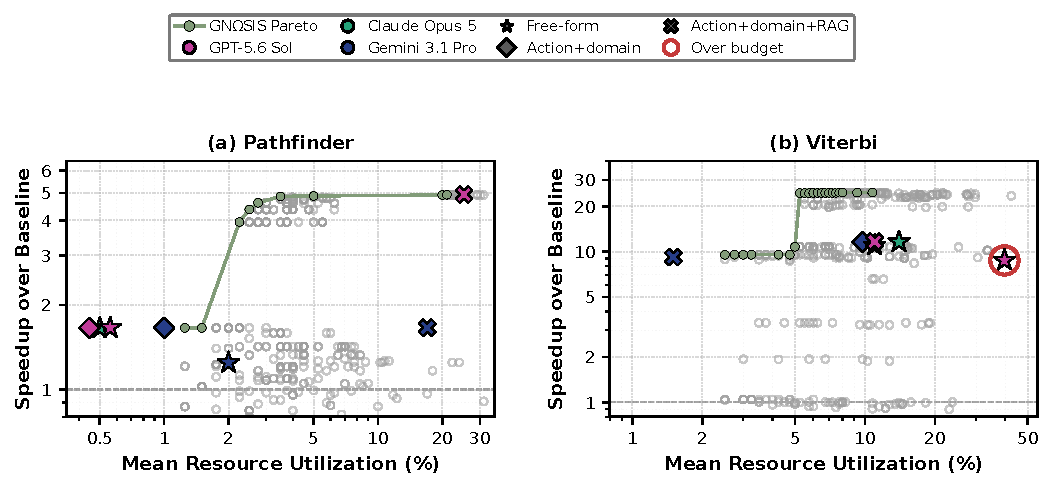
\includegraphics[
        width=0.82\textwidth
    ]{figures/03__Motivation/motivation_pathfinder_viterbi_FINAL.pdf}
    \caption{\textbf{General-purpose LLMs under progressively stronger HLS prompting on Pathfinder and Viterbi.}
    Synthesized designs are compared with the measured GN$\Omega$SIS Pareto frontier~\cite{ferikoglou2026gnomegasis}; red circles denote component-wise resource infeasibility.}
    \label{fig:llm-decoder-limitation}
\end{figure*}

The contrast is not simply a syntax effect. On Pathfinder, the best hosted model reaches $4.94\times$ speedup and lies close to the measured latency-efficient frontier. On Viterbi, the best synthesized hosted-model configuration reaches $11.64\times$, while the measured frontier extends to roughly twice that speedup at comparable or lower resource utilization. 
Moreover, five of the twelve action-structured outputs violate the required assignment schema despite receiving the legal action sites and value domains. Among the thirteen configurations that proceed to synthesis, twelve are component-wise feasible; the remaining Viterbi free-form configuration reaches 103\% LUT utilization. Providing legal action sites therefore removes one source of ambiguity, but does not make prompt-only generation either structurally grounded or reliably constraint aware.


\subsection{Pitfalls of Structure-Agnostic Adaptation}

The three prompting regimes isolate what textual assistance can and cannot supply. Exposing action sites eliminates the need to discover pragma placement; exposing domains provides legal candidate values; and RAG adds explicit HLS knowledge about pipelining, unrolling, partitioning, dependences, and memory bandwidth. These interventions can improve individual decisions---most clearly for GPT-5.6 Sol on Pathfinder---but the information remains an unstructured token sequence. The model must still determine which dependence constrains which loop, which memory object supplies an unrolled computation, and which other directive decisions share that structure.

The missing signal is therefore more specific than generic ''long-range attention.'' HLS decisions need an explicit correspondence between a source action and the compiler relations that determine its hardware effect. This motivates \framework's Stage~2 design: preserve the semantic and target-aware policy learned from source code, but expose each directive decision to compiler-derived memory aligned to the same action identity. The following sections describe how this alignment is constructed and test whether it---rather than additional prompting, output constraints, or model capacity---accounts for the resulting QoR.
\section{\framework: Design Overview}
\label{sec:design-overview}

\begin{figure*}[t]
    \centering
    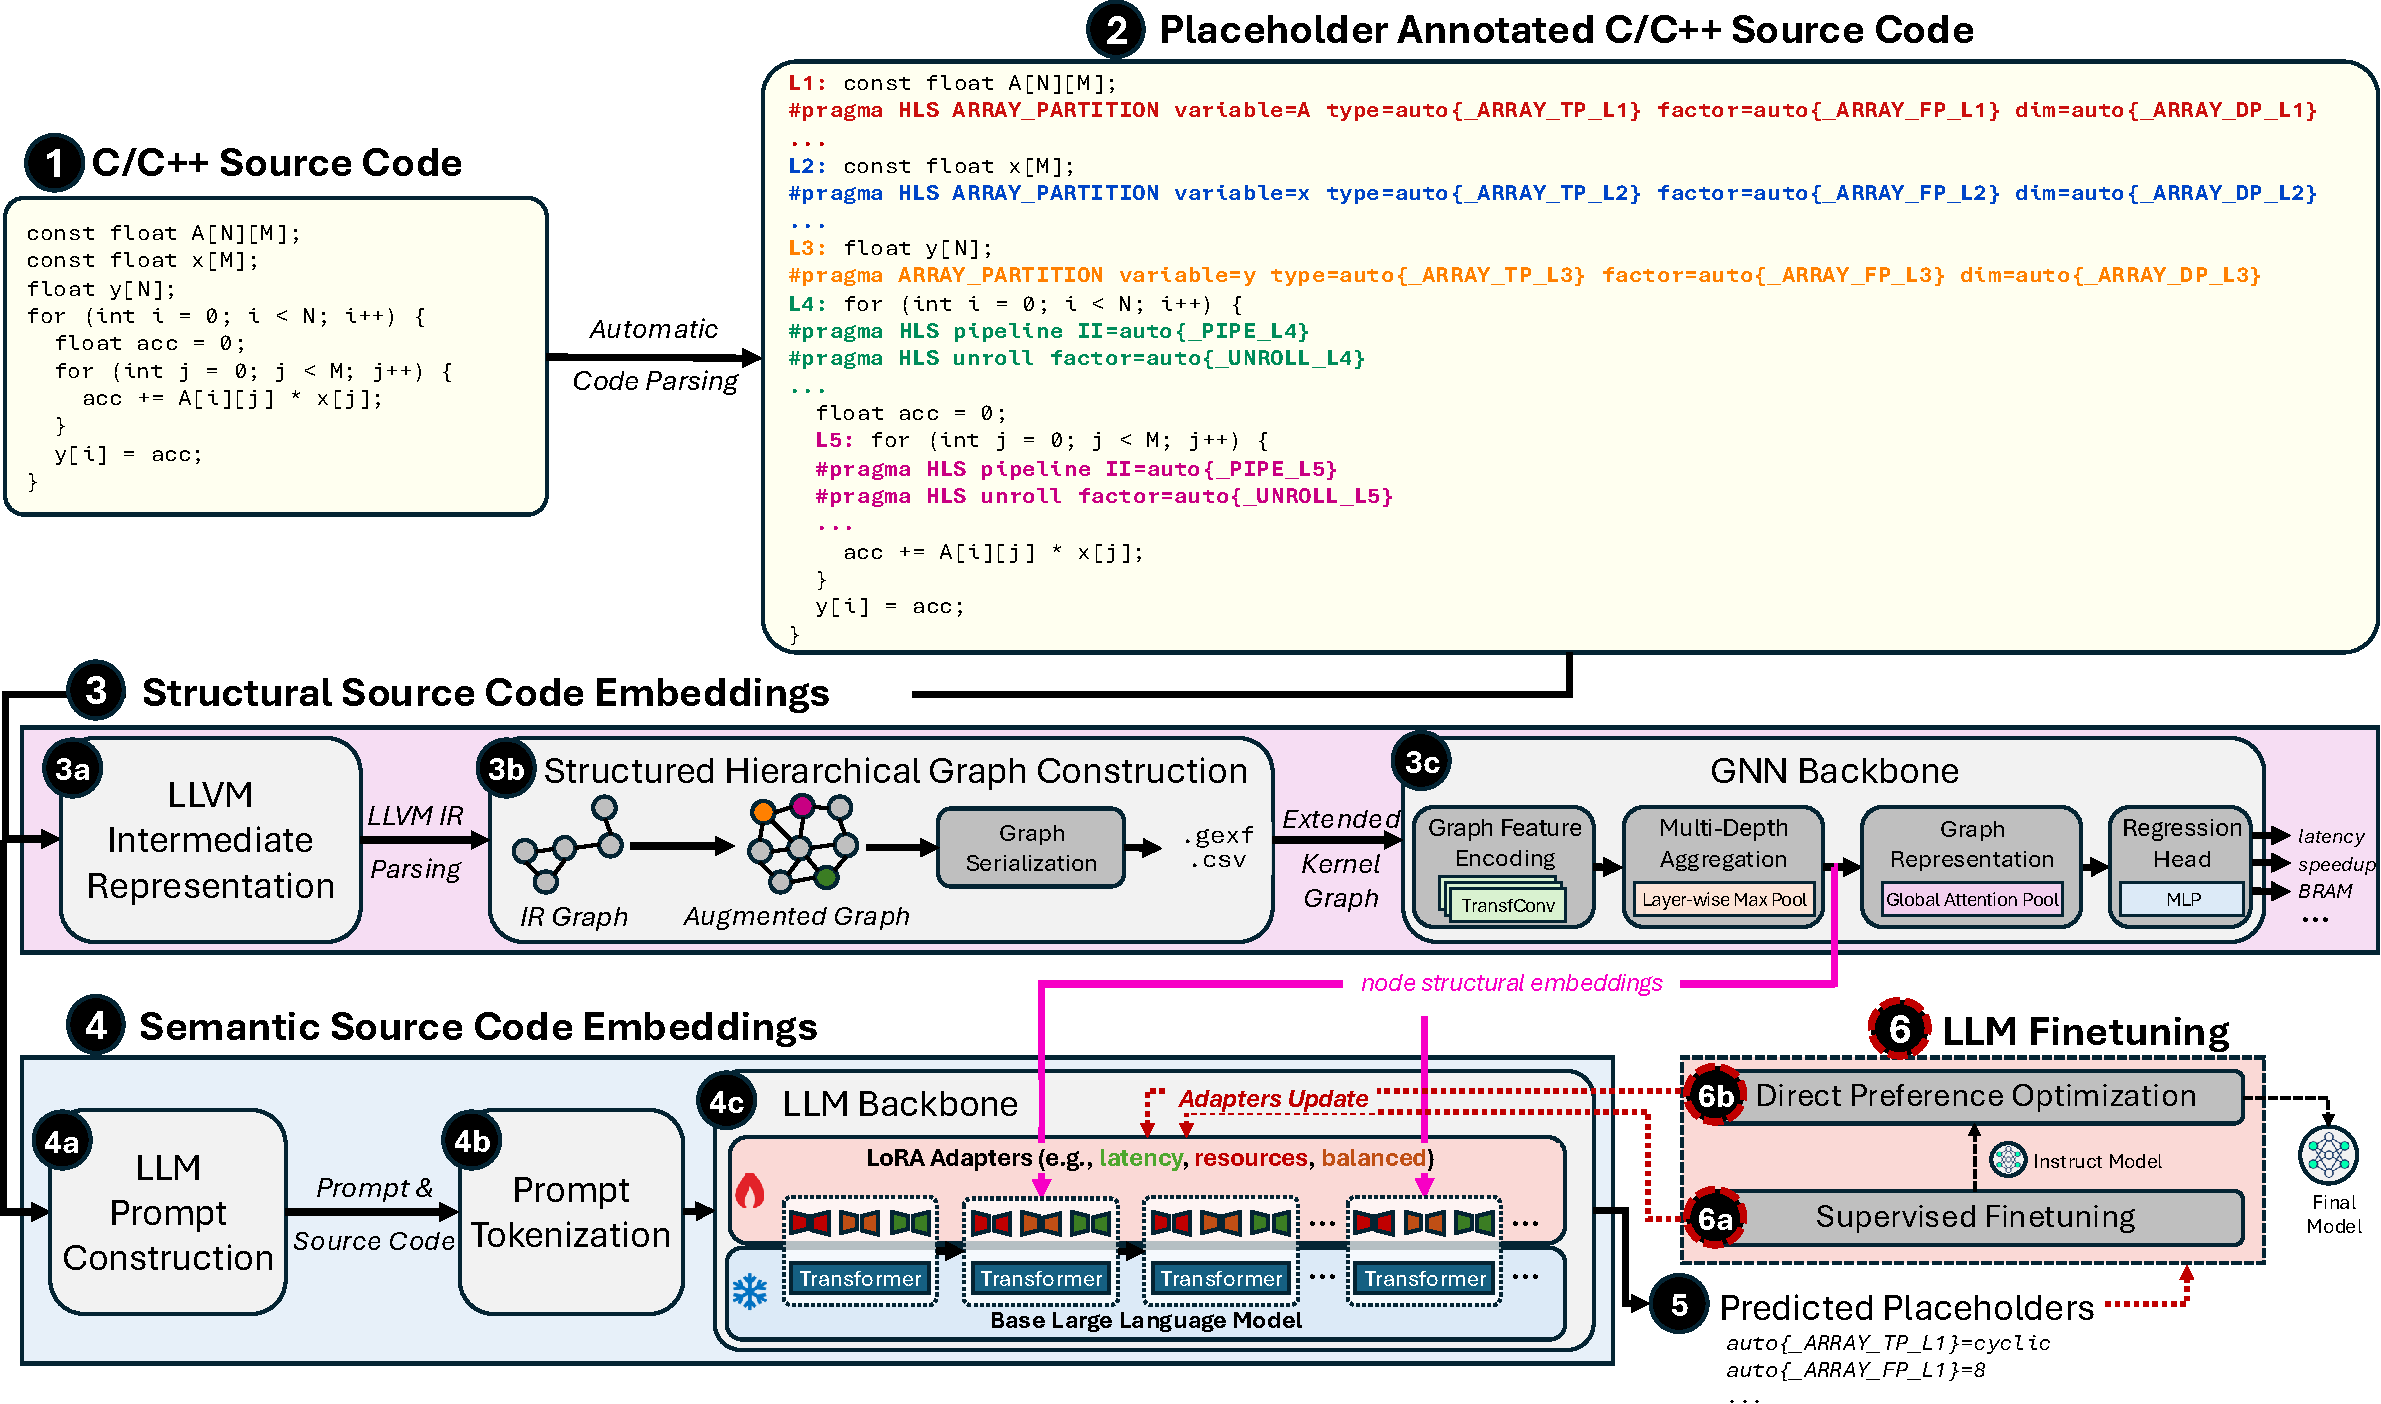
\includegraphics[width=\textwidth]{figures/02__Methodology/Proposed-Architecture-crop.pdf}
    \caption{\framework design overview. Given a C/C++ kernel and target request, \framework identifies directive action points, encodes semantic and compiler-derived structural representations, fuses them through gated cross-attention, and predicts objective-aware pragma values. Cold components denote frozen modules, while hot components denote trainable parts. \EV{should be updated after the figure update}}
    \label{fig:design-overview}
\end{figure*}

\figuretodo{Edit the existing architecture figure :
(1) labeled C/C++ + kernel\_info.txt -> cgeist/Polygeist ->
Affine / SCF / MemRef / Arith / Func MLIR -> deterministic action-aligned graph;
(2) GNN QoR heads as training supervision only, with pre-head action-point embeddings exported to absolute L\_k memory slots;
(3) Stage 1 as target-aware SFT with no structural input;
(4) Stage 2 as frozen Stage 1 plus post-self-attention gated cross-attention at layers 8/16/24/32, with compiler-relational routing and value-only application;
(5) Stage 3 DPO; (6) a small AUTO branch: selector -> supported clock -> ordinary specified-clock SALT-HLS policy.
The prompt box must contain objective, FPGA, BRAM/DSP/FF/LUT budgets, and clock.
Preserve the existing circled workflow and hot/cold visual language.}

% To address the limitations in \S\ref{sec:motivation} \EV{maybe we should close motivation with the overall limitations to have this link for starting to describe our framework}, we propose \framework, a target-conditioned hybrid framework for direct HLS pragma optimization. Training is Pareto-driven in the sense that supervision is constructed from objective-ranked feasible designs within a fixed kernel/device/clock/budget context; inference itself is not a Pareto search. The design follows three principles:

% \begin{enumerate}[leftmargin=*,label=\textbf{(\arabic*)},labelsep=0.3em,topsep=2pt,itemsep=2pt]
%     \item \textbf{Joint structural \& semantic modeling.} \framework combines compiler-derived graph representations with language-model reasoning to capture both program organization and source-level semantics. The GNN encodes explicit relations among loops, regions, values, and memory operations; the LLM interprets source context and the requested optimization target. Gated cross-attention connects the two views at directive decisions. \EV{slightly repetitve?}

%     \item \textbf{Directive-level decision abstraction.} Instead of generating arbitrary HLS code, \framework predicts values for source-derived directive placeholders placed at eligible loop and array action points. The action contract \EV{change action contract} fixes \emph{where} a supported pragma may act and provides a set of accepted directive values including a no-op value which allows the policy to decide whether the action is activated. This substantially reduces syntax/placement errors without implying that every generated configuration is synthesizable or resource-feasible.

%     \item \textbf{Objective- and target-aware optimization.} The policy conditions on one of three objectives---latency, area, or latency-area product (ADP)---and on the target context: target device, available BRAM/DSP/FF/LUT budget, and clock period. The exact objective metric and target protocol are defined in \S\ref{subsec:eval-objectives}. \EV{wwhat are the objective metric and the target protocol?}
% \end{enumerate}

% Figure~\ref{fig:design-overview} presents the end-to-end workflow. Given an input C/C++ kernel (\circled{1}), the framework identifies candidate optimization action points---loops and arrays---and augments them with parameterized directive placeholders (\circled{2}). Each action identity $L_k$ is shared across the source prompt, the compiler graph, and the structural memory, providing a deterministic alignment between the language and graph representations.

% For the \textit{structural representation} (\circled{3}), the source is lowered with cgeist/Polygeist to structured MLIR~\cite{lattner2021mlir}. An edge-aware GNN is trained with QoR supervision \EV{with what loss does the GNN gets trained, with what goal} and exports deterministic action-point embeddings before its prediction heads. \EV{repetition} For the \textit{semantic/target representation} (\circled{4}), a decoder-only code LLM processes the source together with objective, target device, available resource component-wise budget, and clock. Stage~1 learns directive values without structural input; Stage~2 freezes Stage~1 and trains only gated cross-attention at layers 8/16/24/32 using compiler-relational action routing \EV{why at those layers and why compiler-relational routing}. The detailed graph creation and memory extraction are given in \S\ref{sec:detailed-design}.

% Finally, \framework emits one complete directive assignment (\circled{5}). Stage~3, preference-aligns same-context complete design actions without changing the target interface. AUTO-clock adaptation is evaluated as a separate clock-selection component; after selecting a supported period, directive generation uses the unchanged specified-clock policy.

To address the limitations identified in
\S\ref{sec:motivation}, \framework learns a direct mapping from a
source program and deployment request to one complete HLS directive
configuration. Training is Pareto-driven: supervision is selected from
measured designs that are feasible under the same
kernel/device/clock/resource context, whereas deployment performs no
Pareto search.

Figure~\ref{fig:design-overview} summarizes the workflow. A deterministic
source analyzer first identifies the loop and array locations at which
supported HLS decisions may be made and assigns each location a stable
action identity $L_k$ (\circled{1}--\circled{2}). Each action exposes a
finite source-derived value domain, including a no-op choice. The same
action identity is subsequently used by the language representation and
the compiler representation, providing the correspondence required for
structural fusion.

The two model paths are trained separately before they are connected.
On the language path, Stage~1 fine-tunes a decoder-only code model to
predict directive values from the source and target request alone. The
request is
%
\[
\tau=(d,c,\mathbf b),\qquad
\mathbf b=(b_{\rm BRAM},b_{\rm DSP},b_{\rm FF},b_{\rm LUT}),
\]
%
together with the optimization objective. Latency minimizes synthesized
cycles; area minimizes the mean normalized BRAM/DSP/FF/LUT utilization;
and ADP minimizes their latency--area product among designs feasible
under $\tau$ (formal definitions in \S\ref{subsec:eval-objectives}).

In parallel, the structural path raises the pragma-free C/C++ kernel
through cgeist/Polygeist to structured MLIR and converts the resulting
compiler representation into an action-aligned relational graph
(\circled{3}). A separately trained edge-aware GNN receives QoR
supervision from synthesized latency and resource measurements. Its
prediction heads provide training supervision only: the final policy
exports hidden action representations before those heads rather than
using predicted QoR to rank or rerank candidate designs.

Stage~2 freezes the Stage~1 policy and learns gated cross-attention from
directive-value positions to the corresponding structural memory.
Structural fusion is distributed across four decoder depths
(layers 8, 16, 24, and 32), providing repeated access to compiler evidence
while leaving most of the pretrained computation unchanged. Rather than
attending to every action indiscriminately, each directive decision is
restricted to its own structural slot and compiler-related action slots;
the exact relation construction is described in
\S\ref{subsubsec:graph-construction}. Stage~3 finally preference-aligns
complete configurations compared under the same target context.

For a specified-clock request, the resulting system emits one complete
configuration in a single policy invocation (\circled{5}); HLS is used
only afterward for validation and measurement. AUTO-clock operation is a
separate lightweight selector: it first chooses one supported period and
then invokes the unchanged specified-clock policy.


\section{\framework: Detailed Design}
\label{sec:detailed-design}

% What SALT-HLS does, why each design choice exists, compact evidence that the choice behaves as intended

\subsection{Code Parsing \& Action-Space Construction}
\label{subsec:parsing}

\framework converts free-form pragma generation into finite, source-anchored prediction. A deterministic analyzer identifies eligible loop and array actions and assigns each a stable identity $L_k$. Loop actions expose pipeline and unroll values; array actions expose one partition tuple (type, factor, dimension).

\begin{lstlisting}[style=shortlststyle]
<R>L4:</R> for (int i = 0; i < N; i++) {
#pragma HLS pipeline II=<R>auto{_PIPE_L4}</R>
#pragma HLS unroll factor=<R>auto{_UNROLL_L4}</R>
...
\end{lstlisting}

Domains are derived only from source metadata: pipeline uses $\{0,1\}$; unroll uses 0 or supported factors bounded by the loop trip count; and partitioning uses \texttt{none}, \texttt{complete}, \texttt{block}, or \texttt{cyclic} with source-compatible factor/dimension values. Partition fields are decoded and validated jointly, while pipeline and partial unrolling remain independent. Thus \framework constrains directive placement and schema, but not final synthesizability or resource feasibility, which are validated
separately.



\subsection{Structural Source Code Embeddings}
\label{subsec:structural-embeddings}

\framework trains a separate GNN and reuses its hidden representations as structural context for the LLM. The GNN is trained on deterministic structured-MLIR graphs.

% \subsubsection{Structured MLIR Representation}
% \label{subsubsec:mlir}

% The frontend lowers the pragma-free/labeled kernel from \S\ref{subsec:parsing} with cgeist to an MLIR level containing Affine, SCF, memRef, Arith, and Func dialects~\cite{lattner2021mlir,ye2022scalehls}. This abstraction retains structured loop/region information and memory objects before lowering them to flat control flow LLVM IR. Affine operations expose analyzable loop bounds and access functions, SCF retains dynamic structured control, MemRef represents memory objects/views/accesses, Arith represents typed computation, and Func retains call structure. \EV{A little more analytically what each dialect offers, why we chose it}

% The graph builder uses the MLIR Python bindings together with a compiled analysis extension \EV{not very clear sentence for paragraph intro}. It extracts memory effects, view/base-buffer relationships, alias classes, affine dependence information, and affine loop trip counts when provable \EV{more analytically, we do not need another repetition of the previous paragraph}. Unresolved memory-dependence cases are represented conservatively rather than silently treated as independent. 

% \paragraph{Why structured MLIR?}
% This representation is intended to expose compiler relations that are difficult to recover reliably after lowering to flatter control flow. We therefore isolate the representation itself through a controlled comparison: \EV{say explicitly what HARP-Rep and Structured MLIR is, are they GNNs or models or something else trained on different graph representations?}
% \emph{HARP-Rep} uses the recovered HARP-style hierarchical graph, whereas \emph{Structured-MLIR} uses our MLIR graph. They both contain the same
% GN$\Omega$SIS design points, target conditions, directive vectors, QoR labels, family split, learner capacity, optimizer, initialization, and checkpoint rule; only the graph representation and its native features change.

\subsubsection{From C/C++ to Structured MLIR}
\label{subsubsec:mlir}

The structural path lowers the same pragma-free kernel with cgeist/Polygeist to structured MLIR before branch-based LLVM lowering~\cite{lattner2021mlir,moses2021polygeist}. 

The retained MLIR dialects serve complementary roles. \emph{Affine} represents loops and memory accesses whose bounds and index expressions satisfy affine
constraints; these restrictions enable compiler dependence analysis and loop reasoning. \emph{SCF} retains structured loops and conditionals whose
bounds or conditions are general SSA values, covering control that cannot be represented legally in Affine. \emph{MemRef} represents typed memory objects together with loads, stores, and view operations, allowing accesses to be related back to the storage they reference. \emph{Arith} retains the typed computations performed inside those regions, while \emph{Func} preserves function scopes and calls. Keeping Affine and SCF simultaneously therefore avoids two undesirable extremes: forcing non-affine control into an affine model or prematurely lattening all loops into basic-block control flow.

After normalization, the graph builder traverses this structured module and materializes two classes of information: relations already explicit in the IR---such as region containment and SSA def--use---and relations derived by compiler analyses over memory and loop structure. 
Proven memory dependences are encoded explicitly, while unresolved relations remain distinguishable in the graph rather than being treated as evidence of independence; only proven dependence relations are
projected into the Stage~2 action-routing mask.



\subsubsection{From MLIR to an Action-Aligned Graph}
\label{subsubsec:graph-construction}

The normalized module becomes a typed multi-relational graph containing region/loop containment, SSA def--use, memory-object/access, view/base,
and memory/dependence relations. The source identity $L_k$ provides deterministic cross-modal alignment: loop actions anchor to their Affine/SCF loop operation and array actions to the corresponding
array-scope node. The exporter stores that node's GNN state in the absolute memory slot for $L_k$.

The compiler graph is additionally projected to an action-relation mask containing self, nearest labeled loop parent/child, arrays accessed within the loop, and proven dependence-linked actions.
Stage~2 uses this mask to restrict structural attention to compiler-related decisions.

These relations correspond directly to interactions among the supported HLS decisions. Pipelining is constrained by loop-carried computation and memory dependences; unrolling increases the number of operations and memory accesses that may execute concurrently; and array partitioning changes the available memory-level parallelism for the arrays consumed by those operations. Consequently, a useful structural representation must capture not only the loop to which a directive is attached, but also the memory and dependence structure through which that directive affects neighboring decisions.


\begin{figure}[t]
    \centering
    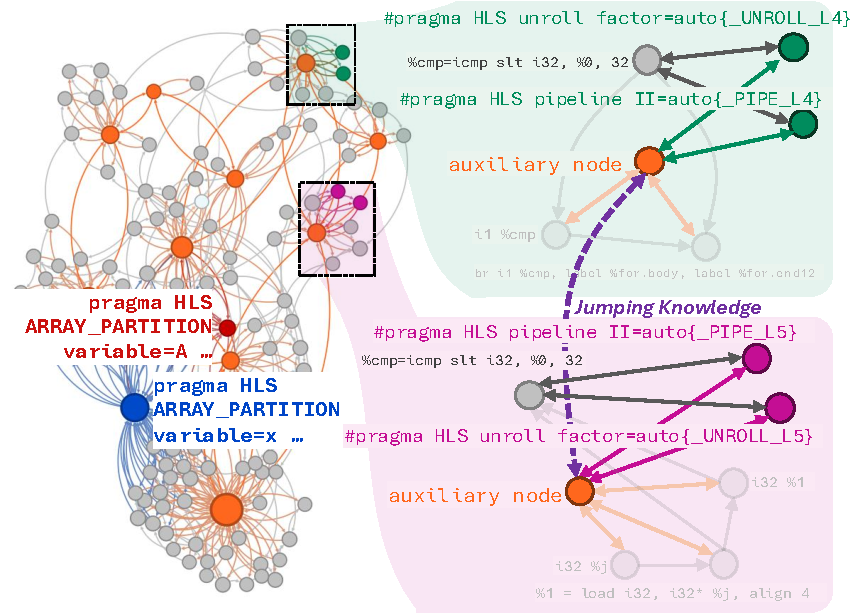
\includegraphics[width=\columnwidth]{figures/02__Methodology/GEMV_Graph-crop.pdf}
    \caption{Structural graph for the GEMV. \figuretodo{\figuretodo{Replace LLVM/icmp nodes with representative Affine/SCF/MemRef operations. Visually distinguish ordinary compiler graph relations from the action-level routing relations consumed by Stage 2. The latter should show self, nearest loop parent/child, array-access scope, and proven dependence forward/reverse.}}}
    \label{fig:gemv-graph}
\end{figure}


A previous version of our work used HARP's hierarchical LLVM graph~\cite{sohrabizadeh2023harp}, we isolate the representation change under a matched GNN control: design points, directive encodings, labels, split, architecture, optimizer, initialization and checkpoint rule are identical; only the graph and native features differ. 

Table~\ref{tab:representation-predictive} reports
graph statistics and selection-relevant ranking metrics. For predictive behavior, Kendall's $\tau_b$ measures how well the surrogate preserves the measured QoR ordering within a target context. Top-1 regret measures the cost of acting on that ranking:
%
\[
R_1=\frac{q(\hat d)}{q(d_{\mathrm{best}})}-1,
\]
%
where $\hat d$ is the design ranked first by the predictor and $d_{\mathrm{best}}$ is the best measured feasible design in the same context. Thus higher $\tau_b$ and lower regret are better.



Both representations align all 544 source actions. Structured MLIR uses 49\% fewer median nodes and 45\% fewer edges while exposing 12 versus 7 relation types; it also improves area/latency $\tau_b$ and reduces top-1 regret by 11.6\%/13.6\%. We therefore adopt it because it is more compact and better aligned with the action-level ranking signal required downstream.

\begin{table}[t]
  \centering
  \caption{\textbf{Matched graph-representation comparison.}
  Structural statistics are median [Q1--Q3] across 55 kernels;
  predictive metrics are macro-averaged across 24 validation
  kernel/device/clock groups (13,011 design points).}
  \label{tab:representation-predictive}

  \scriptsize
  \setlength{\tabcolsep}{3.0pt}
  \renewcommand{\arraystretch}{1.05}

  \begin{tabular}{lrr}
    \toprule
    \textbf{Metric} &
    \textbf{HARP-Rep} &
    \textbf{Structured MLIR} \\
    \midrule

    \multicolumn{3}{l}{\emph{Representation audit}} \\
    Action points aligned
        & 544/544 & 544/544 \\
    Nodes/kernel
        & 645 [361--1008] & 328 [159--542] \\
    Edges/kernel
        & 2,283 [1,269--3,684] & 1,267 [624--2,646] \\
    Relation types/kernel
        & 7 [6--7] & 12 [11--12] \\
    R/M/C/D/U edges
        & 0/0/0/0/0 & 24/66/3/5/12 \\

    \midrule
    \multicolumn{3}{l}{\emph{Selection-relevant prediction}} \\
    Area Kendall $\tau_b$ $\uparrow$
        & 0.284 & \textbf{0.316} \\
    Latency Kendall $\tau_b$ $\uparrow$
        & 0.201 & \textbf{0.224} \\
    Area top-1 regret $\downarrow$
        & 4.232 & \textbf{3.742} \\
    Latency top-1 regret $\downarrow$
        & 0.404 & \textbf{0.349} \\

    \bottomrule
  \end{tabular}

  \vspace{1pt}
  \parbox{0.98\columnwidth}{\scriptsize
  R/M/C/D/U denote region, memory-access, loop-carried,
  proven-dependence, and unresolved-dependence relations.
  A zero indicates that the relation is not encoded as a distinct
  edge class; it does not imply that no related information can be
  inferred transitively from the original graph.}
\end{table}






\subsubsection{QoR-Supervised GNN and Structural Memory}
\label{subsubsec:gnn-backbone}

Each graph is encoded by four edge-aware TransformerConv layers with 64-dimensional states and JK-max aggregation~\cite{xu2018jumping};
graph pooling and latency/resource heads are used only during GNN training. QoR supervision encourages the representation to preserve hardware-relevant dependence, parallelism, and memory information.

At export, prediction heads and directive-value features are removed.
For each $L_k$, we concatenate a 64-D early-layer state, preserving local compiler context, with the 64-D JK state, capturing a wider receptive field. Training-set centering/RMS normalization yields the 128-D pragma-free structural memory used by Stage~2. Device, clock, budget, and objective conditioning remain in the language policy.




\subsection{Target-Conditioned Structural-Semantic Policy}
\label{subsec:llm-backbone}

\framework learns $p(\mathbf d\mid\text{source},o,\tau)$ over the source-derived action points. Stage~1 learns the target/objective-conditioned semantic policy; Stage~2 freezes it and learns gated access to action-aligned compiler memory.


\subsubsection{LLM Prompt Construction}
\label{subsubsec:prompt}

For each action $L_k$, \texttt{<SRC\_Lk>} marks its source location and \texttt{<Lk>} anchors the corresponding output assignments.
Assignment names and order are fixed; the model predicts only directive values, and $L_k$ also serves as the Stage~2 routing identity.
The prompt supplies objective, FPGA, clock, and component-wise BRAM/DSP/FF/LUT budgets as both counts and fractions of device capacity. During Stage~1, the same kernel/device/clock case is presented under multiple budgets, with supervision drawn only from
designs feasible under all four limits.

Among feasible candidates, the objective-specific ranking determines the measured configuration used as supervision; the ranking and budget-sampling policy are detailed in \S\ref{subsec:eval-data}.



\subsubsection{Target-Aware Conditioning}
\label{subsubsec:target-conditioning}

For specified-clock inference, the deployment target is
\[
\tau=(d,c,\mathbf b),\qquad
\mathbf b=(b_{\rm BRAM},b_{\rm DSP},b_{\rm FF},b_{\rm LUT}).
\]
Stage~1 minimizes cross-entropy only at directive value positions, conditioned jointly on source, objective $o$, and $\tau$; fixed anchors and directive syntax are not supervised. Thus identical source code under different clocks or budgets forms different conditional examples: a policy that ignores $\tau$ cannot fit conflicting target-specific assignments. Stage~2 preserves this interface and adds only structural evidence.

% \begin{table}[t]
%     \centering
%     \caption{Target responsiveness of GPT-5.6 Sol, the strongest general-purpose LLM in our evaluation, on GAN. Each row changes only
%     the indicated target attribute relative to C0. Speedup is measured
%     against the pragma-free baseline synthesized for the same device and
%     clock. $\Delta$Dir. denotes the fraction of the 25 directive-value
%     fields changed relative to C0.}
%     \label{tab:gpt_target_responsiveness}
%     \scriptsize
%     \setlength{\tabcolsep}{3.0pt}
%     \renewcommand{\arraystretch}{1.05}
%     \begin{tabular}{lrrrr}
%         \toprule
%         \textbf{Target} &
%         \textbf{Speedup} &
%         \textbf{Res. (\%)} &
%         \textbf{$\Delta$Dir.} &
%         \textbf{Feas.} \\
%         \midrule
%         C0: Latency, ZCU104, 10\,ns
%             & 149.96$\times$ & 26.73 & 0\%  & Yes \\
%         Objective $\rightarrow$ Area
%             &   1.00$\times$ &  1.20 & 60\% & Yes \\
%         Objective $\rightarrow$ ADP
%             & 125.80$\times$ &  6.09 & 20\% & Yes \\
%         Budget $\rightarrow$ 15\%
%             &  78.72$\times$ &  8.45 & 20\% & No$^\dagger$ \\
%         Device $\rightarrow$ U200
%             & 155.13$\times$ &  5.87 & 12\% & Yes \\
%         Clock $\rightarrow$ 3.33\,ns
%             & 172.70$\times$ & 26.63 & 12\% & Yes \\
%         \bottomrule
%     \end{tabular}

%     \vspace{1pt}
%     \parbox{\columnwidth}{\scriptsize
%     $^\dagger$The synthesized design exceeds the requested tight
%     component-wise budget only in LUTs
%     ($1.036\times$ the allowed LUT budget).}
% \end{table}

\begin{figure}[t]
    \centering
    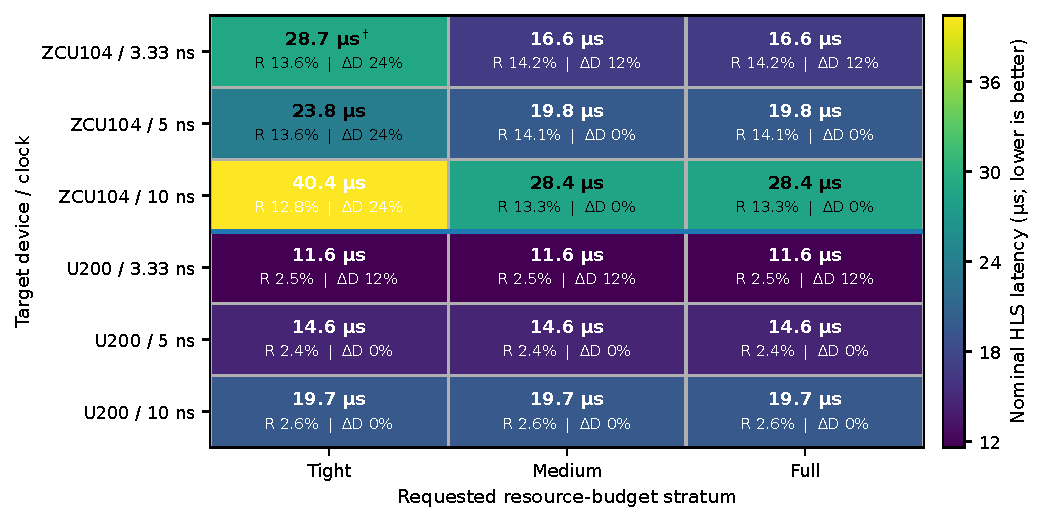
\includegraphics[
        width=0.97\columnwidth
    ]{figures/02__Methodology/target_conditioning_heatmap.pdf}
    \caption{
        \textbf{Target conditioning across device, clock, and resource
        requests on GAN.}
        Each synthesized target reports latency (top), mean resource
        utilization $R$, and the directive change $\Delta D$ relative to
        ZCU104/10\,ns/full. Lower latency is better; $\dagger$ denotes a
        missed requested clock.
    }
    \Description{
        Heatmap of eighteen synthesized SALT-HLS configurations across
        two FPGA devices, three clock periods, and three resource-budget
        strata.
    }
    \label{fig:target-conditioning}
\end{figure}

Figure~\ref{fig:target-conditioning} confirms that these target fields affect the emitted policy. On ZCU104/10\,ns, tightening the budget changes 24\% of directive fields and trades latency (28.4$\rightarrow$40.4\,$\mu$s) for lower resource use; changing clock similarly changes the assignment. Conversely, the three U200 budgets select the same directives when the limits are non-binding, showing that the policy does not change merely because a prompt number changes. The missed 3.33\,ns case also emphasizes that target conditioning does not replace post-generation HLS validation.



\subsubsection{LLM Backbone \& Structural Embeddings Fusion}
\label{subsubsec:structural-fusion}

Stage~2 turns the target-conditioned language policy into an action-grounded structural policy. The decoder hidden state provides the semantic and target-aware query, whereas the action-aligned GNN memory of \S\ref{subsubsec:gnn-backbone} provides compiler-derived keys and values. The Stage~1 policy is frozen: Stage~2 learns only how structural evidence should correct an already functional directive policy.

For a directive RHS position associated with action $L_k$, the structural update can be written schematically as
%
\[
\tilde{\mathbf h}_t =
\mathbf h_t +
\tanh(g)\,
\mathrm{XAttn}(\mathbf h_t,\mathbf M;\mathbf A_k),
\qquad t\in\mathcal R_k .
\]
%
where $\mathbf h_{\mathrm{SA}}$ is the representation after causal self-attention, $\mathbf M$ is the structural-memory bank, $\mathbf A_k$ is the compiler-derived routing mask for $L_k$, and $g$ is a learned residual gate. Structural fusion is therefore selective in two independent ways: only directive-value positions receive the update, and each such position can inspect only structural slots related to its current action.

Cross-attention is applied after the self-attention residual and before the block's feed-forward transformation. This ordering first lets the causal decoder combine source, objective, and target context, then lets that contextualized directive state query compiler memory before further local transformation. The residual gate is initialized at zero, so inserting the structural path initially reproduces the frozen Stage~1 policy and structural corrections are introduced only as training opens the gate.

DeepSeek-Coder-6.7B contains 32 decoder layers; we insert structural fusion after every eighth layer, yielding four interaction points distributed over the backbone. This provides repeated access to compiler evidence without modifying every pretrained block. During Stage~2, the backbone, Stage~1 LoRA, and special-token embeddings remain frozen; only structural cross-attention and its gates are optimized. We evaluate the sensitivity to fusion frequency below and report the remaining architectural hyperparameters in \S\ref{subsec:eval-training}.


\paragraph{Does aligned structural memory matter?}
We test the structural pathway with a fixed-checkpoint intervention rather than retraining separate models. The same frozen ADP policy is evaluated on 18 post-freeze Kalman contexts spanning device, clock, and resource requests. The contexts are selected without QoR information: within each device/clock group we take three evenly spaced quantiles of requested resource fraction. Across interventions we keep the backbone, Stage~1 LoRA, Stage~2 cross-attention weights, decoding rule, and target request identical; only the memory presented to Stage~2 changes.

\emph{Zero} preserves the Stage~2 architecture and routing masks but sets the structural values to zero, testing whether the added fusion machinery alone changes the policy. \emph{Deranged} preserves the same within-kernel set of non-zero structural vectors but applies a deterministic permutation with no action retaining its original vector, breaking the correspondence between $L_k$ and its compiler representation while preserving memory magnitude and cardinality. \emph{Aligned} supplies each $L_k$ with its correct MLIR-derived memory. The comparison therefore separates (i) adding a structural pathway, (ii) supplying arbitrary non-zero side information, and (iii) supplying compiler information under the correct action identity.

Table~\ref{tab:memory-ablation} shows a representative ZCU104/10\,ns synthesis; speedups use the same pragma-free baseline and resource entries are percentages of device capacity in [BRAM, DSP, FF, LUT] order.

\begin{table}[t]
    \centering
    \caption{\textbf{Fixed-checkpoint structural-memory intervention on a
    representative Kalman target} (ZCU104, 10\,ns, full device budget).}
    \label{tab:memory-ablation}
    \scriptsize
    \setlength{\tabcolsep}{3.0pt}
    \renewcommand{\arraystretch}{1.08}

    \begin{tabular}{lccr}
        \toprule
        \textbf{Policy} &
        \textbf{Speedup} &
        \textbf{Feas.} &
        \textbf{[BRAM,DSP,FF,LUT] (\%)} \\
        \midrule
        Stage 1
          & 1.23$\times$  & No  & [183.97,0.12,1.19,8.14] \\
        Stage 2--Zero
          & 1.23$\times$  & No  & [183.97,0.12,1.19,8.14] \\
        Stage 2--Deranged
          & 19.43$\times$ & No  & [183.97,0.23,1.57,8.30] \\
        Stage 2--Aligned
          & \textbf{20.70$\times$} & \textbf{Yes}
          & [96.79,0.23,1.53,8.26] \\
        \bottomrule
    \end{tabular}
\end{table}

The representative synthesis illustrates the three controls clearly.
Zero memory exactly reproduces Stage~1 (1.23$\times$ and 183.97\% BRAM), showing that the additional cross-attention topology alone does not explain the gain. Deranged memory strongly changes the policy and reaches 19.43$\times$ speedup, confirming that the structural branch is active, but it retains the catastrophic 183.97\% BRAM allocation. Restoring the correct action--memory correspondence preserves the acceleration (20.70$\times$) while reducing BRAM to 96.79\%, making the configuration feasible. Thus the useful effect in this case is not simply ``more side
information'': the structural evidence must be associated with the action whose directive is being predicted. 



\paragraph{LLM backbone capacity.}

% \begin{figure}[t]
%     \centering
%     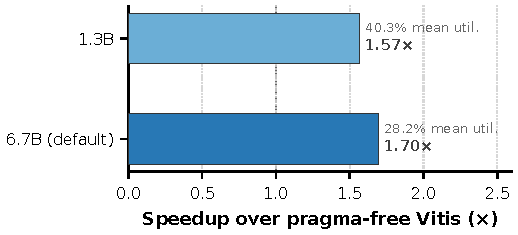
\includegraphics[
%         width=0.96\columnwidth
%     ]{figures/02__Methodology/backbone_capacity_sensitivity.pdf}
%     \caption{
%         \textbf{Backbone-capacity sensitivity on JPEG.}
%         We compare the production 6.7B backbone with a 1.3B variant
%         while retaining the same latency-oriented SALT-HLS task.
%         Labels report measured speedup and mean BRAM/DSP/FF/LUT
%         utilization. The larger backbone improves synthesized QoR while
%         requiring a smaller hardware resource footprint.
%     }
%     \Description{
%         Horizontal bar chart comparing 1.3B and 6.7B SALT-HLS
%         backbones on JPEG by synthesized speedup over pragma-free Vitis.
%         Labels additionally report mean FPGA resource utilization.
%     }
%     \label{fig:backbone-capacity}
% \end{figure}

\EV{small paragraph explaining the backbone capacity experiment, why did we choose this experimental setup (covariance), what conclusions can we draw from it, results with numbers when we insert figure}


\paragraph{Cross-attention placement}

\EV{small paragraph explaining the xattn placement experiment, why did we choose this experimental setup (jpeg), what conclusions can we draw from it, results with numbers when we insert figure}

\EV{Our gains come from SALT architecture rather than the backbone size}


\subsubsection{Objective-Aware Specialization}
\label{subsubsec:peft}

Target conditioning specifies the deployment constraints, whereas the objective selects the preferred feasible trade-off. We therefore share
the code backbone and target interface but maintain separate LoRA adapters~\cite{hu2022lora} for latency, area, and ADP; at inference, $o$ selects the corresponding adapter. This avoids collapsing conflicting objective updates into one policy without duplicating the backbone.


\paragraph{Preference alignment.}
Stage~3 completes the \framework training pipeline by aligning the structurally grounded Stage~2 policy with whole-design hardware preferences.
We construct preference pairs from complete directive configurations evaluated under the same kernel, device, clock, resource budget, and objective; the
chosen design has better measured objective QoR than the rejected one. Holding the target context fixed ensures that the preference signal reflects the directive configuration itself rather than an easier deployment setting. 
We then apply reference-based DPO~\cite{rafailov2023dpo}, which increases the relative likelihood of the preferred complete configuration without training a separate reward model. This whole-design objective complements the token-level supervision of Stages~1--2: it captures interactions among pipeline, unroll, and partition decisions that cannot be attributed reliably to individual directive fields. During Stage~3, the Stage~1 semantic LoRA remains fixed while the structural-fusion parameters are refined, preserving the learned target-conditioned policy while aligning its final decisions with measured hardware preference.



\subsubsection{Automatic Clock Selection}
\label{subsubsec:auto-clock}

If the clock is unspecified, a separate selector chooses $\hat c\in\mathcal C(d)$ from the device-defined measured clock menu using the frozen structural memory and target/objective context.
Training labels select the clock whose best feasible same-context design minimizes the requested objective. \framework then rewrites the request as $(d,\hat c,\mathbf b,o)$ and invokes the ordinary specified-clock policy once. \textsc{Auto} therefore adds one discrete choice rather than an iterative clock--pragma search.\EV{mention the clock accuracy}
\section{Evaluation Methodology}
\label{sec:evaluation-methodology}

\subsection{Dataset, Split, and Targets}
\label{subsec:eval-data}

We train on the GN$\Omega$SIS corpus~\cite{ferikoglou2026gnomegasis},
which contains approximately 219K Vitis HLS design points.
The source-resolvable SALT-HLS subset contains 150,026 measured
configurations from 55 kernels. Language-policy training retains two
FPGA targets---ZCU104 (\texttt{xczu7ev-ffvc1156-2-e}) and Alveo U200
(\texttt{xcu200-fsgd2104-2-e})---at 3.33, 5, and 10\,ns.
Their full [BRAM$_{18K}$, DSP, FF, LUT] capacities are
[624, 1728, 460800, 230400] and
[4320, 6840, 2364480, 1182240], respectively.

We freeze one family-disjoint split (seed 123) for all learned
components: 130,310 rows from 50 kernels/18 families for training,
13,011 rows from four kernels/three families for validation, and
6,705 rows from the Serrano Kalman family as the locked test set.
No test or external-evaluation workload contributes to parameter
updates or checkpoint selection. The structural GNN follows the same
family holdout but receives QoR supervision only on XCZU7EV/10\,ns,
deliberately leaving device, clock, and budget conditioning to the
language policy.

For each training $(\text{kernel},\text{device},\text{clock})$ case,
we construct 16 component-wise resource-budget requests with a 5\%
minimum per resource. A request is retained only if at least three
measured designs satisfy all four limits; up to 24 same-context
candidates form the objective pool, from which the best
objective-ranked feasible design supplies supervision. Directive
domains depend only on source metadata and are therefore independent
of which measured designs survive a budget.

Unless stated otherwise, end-to-end QoR is evaluated on ZCU104/10\,ns at full device capacity. We deliberately construct the nine-kernel evaluation suite as a heterogeneous stress set rather than drawing all workloads from a single benchmark family. It combines two GN$\Omega$SIS-origin applications excluded from policy training (Kalman and 3D Rendering) with seven workloads from external sources/suites: GAN, PolyBench Covariance, Jacobi-2D, SYR2K, and TRMM, and CHStone AES and JPEG. This composition introduces both provenance and structural shifts while covering dense neural computation, memory-constrained filtering, regular matrix and stencil
nests, cryptography, codec/control-intensive code, and graphics.
The resulting kernels expose 3-21 directive action sites and markedly different baseline resource pressure and optimization headroom.
Consequently, the evaluation does not assume that kernel size or the number of available transformations predicts optimization difficulty;
instead, it tests whether SALT-HLS can select useful policies across different dependence structures, memory constraints, and opportunities for parallelism.

We separately test zero-shot target transfer on four deliberately
contrasting kernels---compute-parallel GAN, control- and buffer-intensive JPEG, regular affine Covariance, and memory-constrained Kalman.
Starting from ZCU104/10\,ns, we independently change either the clock to the unseen 6.67\,ns period or the device to the unseen Alveo U50 while holding the other target dimension fixed. The 6.67\,ns point ($\approx$150\,MHz) lies between the 10 and 5\,ns clocks observed during training and therefore tests interpolation to an unseen timing target;
U50 tests device transfer at the familiar 10\,ns clock. Neither target participates in training or model selection.


\subsection{Objectives and Metrics}
\label{subsec:eval-objectives}
\label{subsec:eval-metrics}

For resource $r\in\{\mathrm{BRAM},\mathrm{DSP},\mathrm{FF},\mathrm{LUT}\}$,
we define normalized utilization
$u_r(d)=100R_r(d)/C_r$ and the training-time area proxy
%
\[
A(d)=\frac{1}{4}\sum_r u_r(d).
\]
%
A design is feasible iff every measured resource satisfies its
requested component-wise budget. The three policies minimize,
respectively, synthesized latency $L$, area proxy $A$, and
ADP $L\,A$; the implementation ranks ADP as
$\log_2 L+\log_2 A$, which is order-equivalent for positive values.
$A$ is a ranking proxy rather than a claim of physical silicon area,
so resource results always report BRAM, DSP, FF, and LUT separately.

For same-target experiments, speedup is
$L_{\mathrm{base}}/L_{\mathrm{method}}$ relative to the pragma-free
Vitis implementation under the same part and requested clock, and
aggregates use the geometric mean. For zero-shot clock/device transfer,
where a same-target pragma-free baseline is unavailable, we instead use
nominal execution time $T=Lc$ and report
$T_{\mathrm{ZCU104},10\mathrm{ns}}/T_{\mathrm{transfer}}$.
We distinguish malformed/materialization failures, HLS-synthesis
failures, and synthesized but resource-infeasible designs rather than
collapsing them into one failure rate.


\subsection{Training Protocol}
\label{subsec:eval-training}

\paragraph{Stage 1.}
We use the pinned DeepSeek-Coder-6.7B base model~\cite{guo2024deepseekcoder}
with 4-bit NF4 quantization. Each objective has a LoRA
adapter~\cite{hu2022lora} with rank 8, $\alpha=16$, dropout 0.1,
and attention-projection targets. Training uses a maximum sequence
length of 7168, batch size 1 with eight-step gradient accumulation,
two epochs, LoRA learning rate $1.5\times10^{-5}$, special-token
learning rate $5\times10^{-6}$, cosine decay, 5\% warm-up, and seed 123.
Only directive RHS values with non-singleton source domains contribute
to the prediction loss.

\paragraph{Structural encoder and Stage 2.}
The structured-MLIR GNN uses the architecture of
\S\ref{subsubsec:gnn-backbone} with 403-D node and 82-D edge features.
It is trained on standardized absolute latency/resource targets using
Smooth-$L_1$ loss ($\beta=0.5$), with rank and resource auxiliary
weights 0.05 and 0.10, respectively; the learning rate is
$3\times10^{-5}$ for at most 40 epochs. The validation-selected
epoch-9 checkpoint exports the pragma-free multiscale action memory
used by all Stage~2 policies.

Stage~2 initializes from the matching objective-specific Stage~1
adapter and freezes the backbone, LoRA, and special-token embeddings.
Only the four compiler-routed cross-attention modules and gates are
trained---8.68M parameters, approximately 0.13\% of the 6.76B-parameter
model. We use effective batch size 8, cosine decay with 5\% warm-up,
and at most three epochs; objective-specific learning rates and the
final checkpoint are selected exclusively on the frozen validation
split.

\paragraph{Stage 3.}
Stage~3 completes SALT-HLS with reference-based DPO
~\cite{rafailov2023dpo} over whole-design, same-context preference
pairs. Pairs share kernel, device, clock, budget, objective, and
supervised schema and differ at the semantic-action level; their order
is determined by measured objective QoR. We use $\beta=0.5$, a 0.02
chosen-NLL/SFT anchor, effective batch size 8, and 40 optimization
steps. The Stage~1 LoRA remains frozen; cross-attention and its gates
are refined with learning rate $2\times10^{-5}$.


\subsection{Baselines and Synthesis Protocol}
\label{subsec:eval-baselines}

The motivation study evaluates GPT-5.6 Sol, Claude Opus 5, and
Gemini 3.1 Pro Preview in one-pass \emph{free-form},
\emph{action+domain}, and \emph{action+domain+RAG} regimes.
The action-matched variants receive the same source action sites,
finite RHS domains, target constraints, and objective as SALT-HLS;
RAG adds general HLS guidance but no GN$\Omega$SIS QoR,
Pareto configurations, SALT-HLS outputs, or synthesis feedback.

For end-to-end comparison we use AutoDSE
~\cite{sohrabizadeh2020autodse}, HARP-DSE
~\cite{sohrabizadeh2023harp}, LIFT~\cite{prakriya2025lift},
and CollectiveHLS~\cite{ferikoglou2024collectivehls} on common
workloads, and additionally compare with the strongest
action+domain+RAG general-purpose LLM on GAN and Kalman.
We report only method--kernel pairs for which a meaningful common
experiment is available; missing experiments are marked
\emph{n/e} or \emph{TBD} rather than imputed.

Unless explicitly stated otherwise, all reported accelerator QoR is
obtained with Vitis HLS 2021.1 under the requested FPGA part and clock.
The pragma-free implementation synthesized under the same target is
the reference for same-target speedup. Finally, we distinguish
\emph{online HLS feedback}---synthesis whose result affects configuration
selection---from synthesis used only to validate the final emitted design.
SALT-HLS uses no online HLS feedback during directive selection and one final synthesis for QoR measurement.
\section{Experimental Results}
\label{sec:results}

% does the complete system actually produce good hardware, generalize, remain valid, and beat alternatives?

We organize the evaluation around four questions:
(1) does the direct policy produce high-quality feasible designs on held-out and external kernels;
(2) does changing the deployment request move the synthesized design in the intended direction;
(3) does correctly aligned compiler memory improve the policy beyond task-specific fine-tuning and a generic side channel; and
(4) how does the resulting policy compare with LLM and DSE baselines in validity, QoR, and online HLS cost?


\subsection{End-to-End Evaluation and Generalization}
\label{subsec:salt-evaluation}


\begin{figure*}[t]
    \centering
    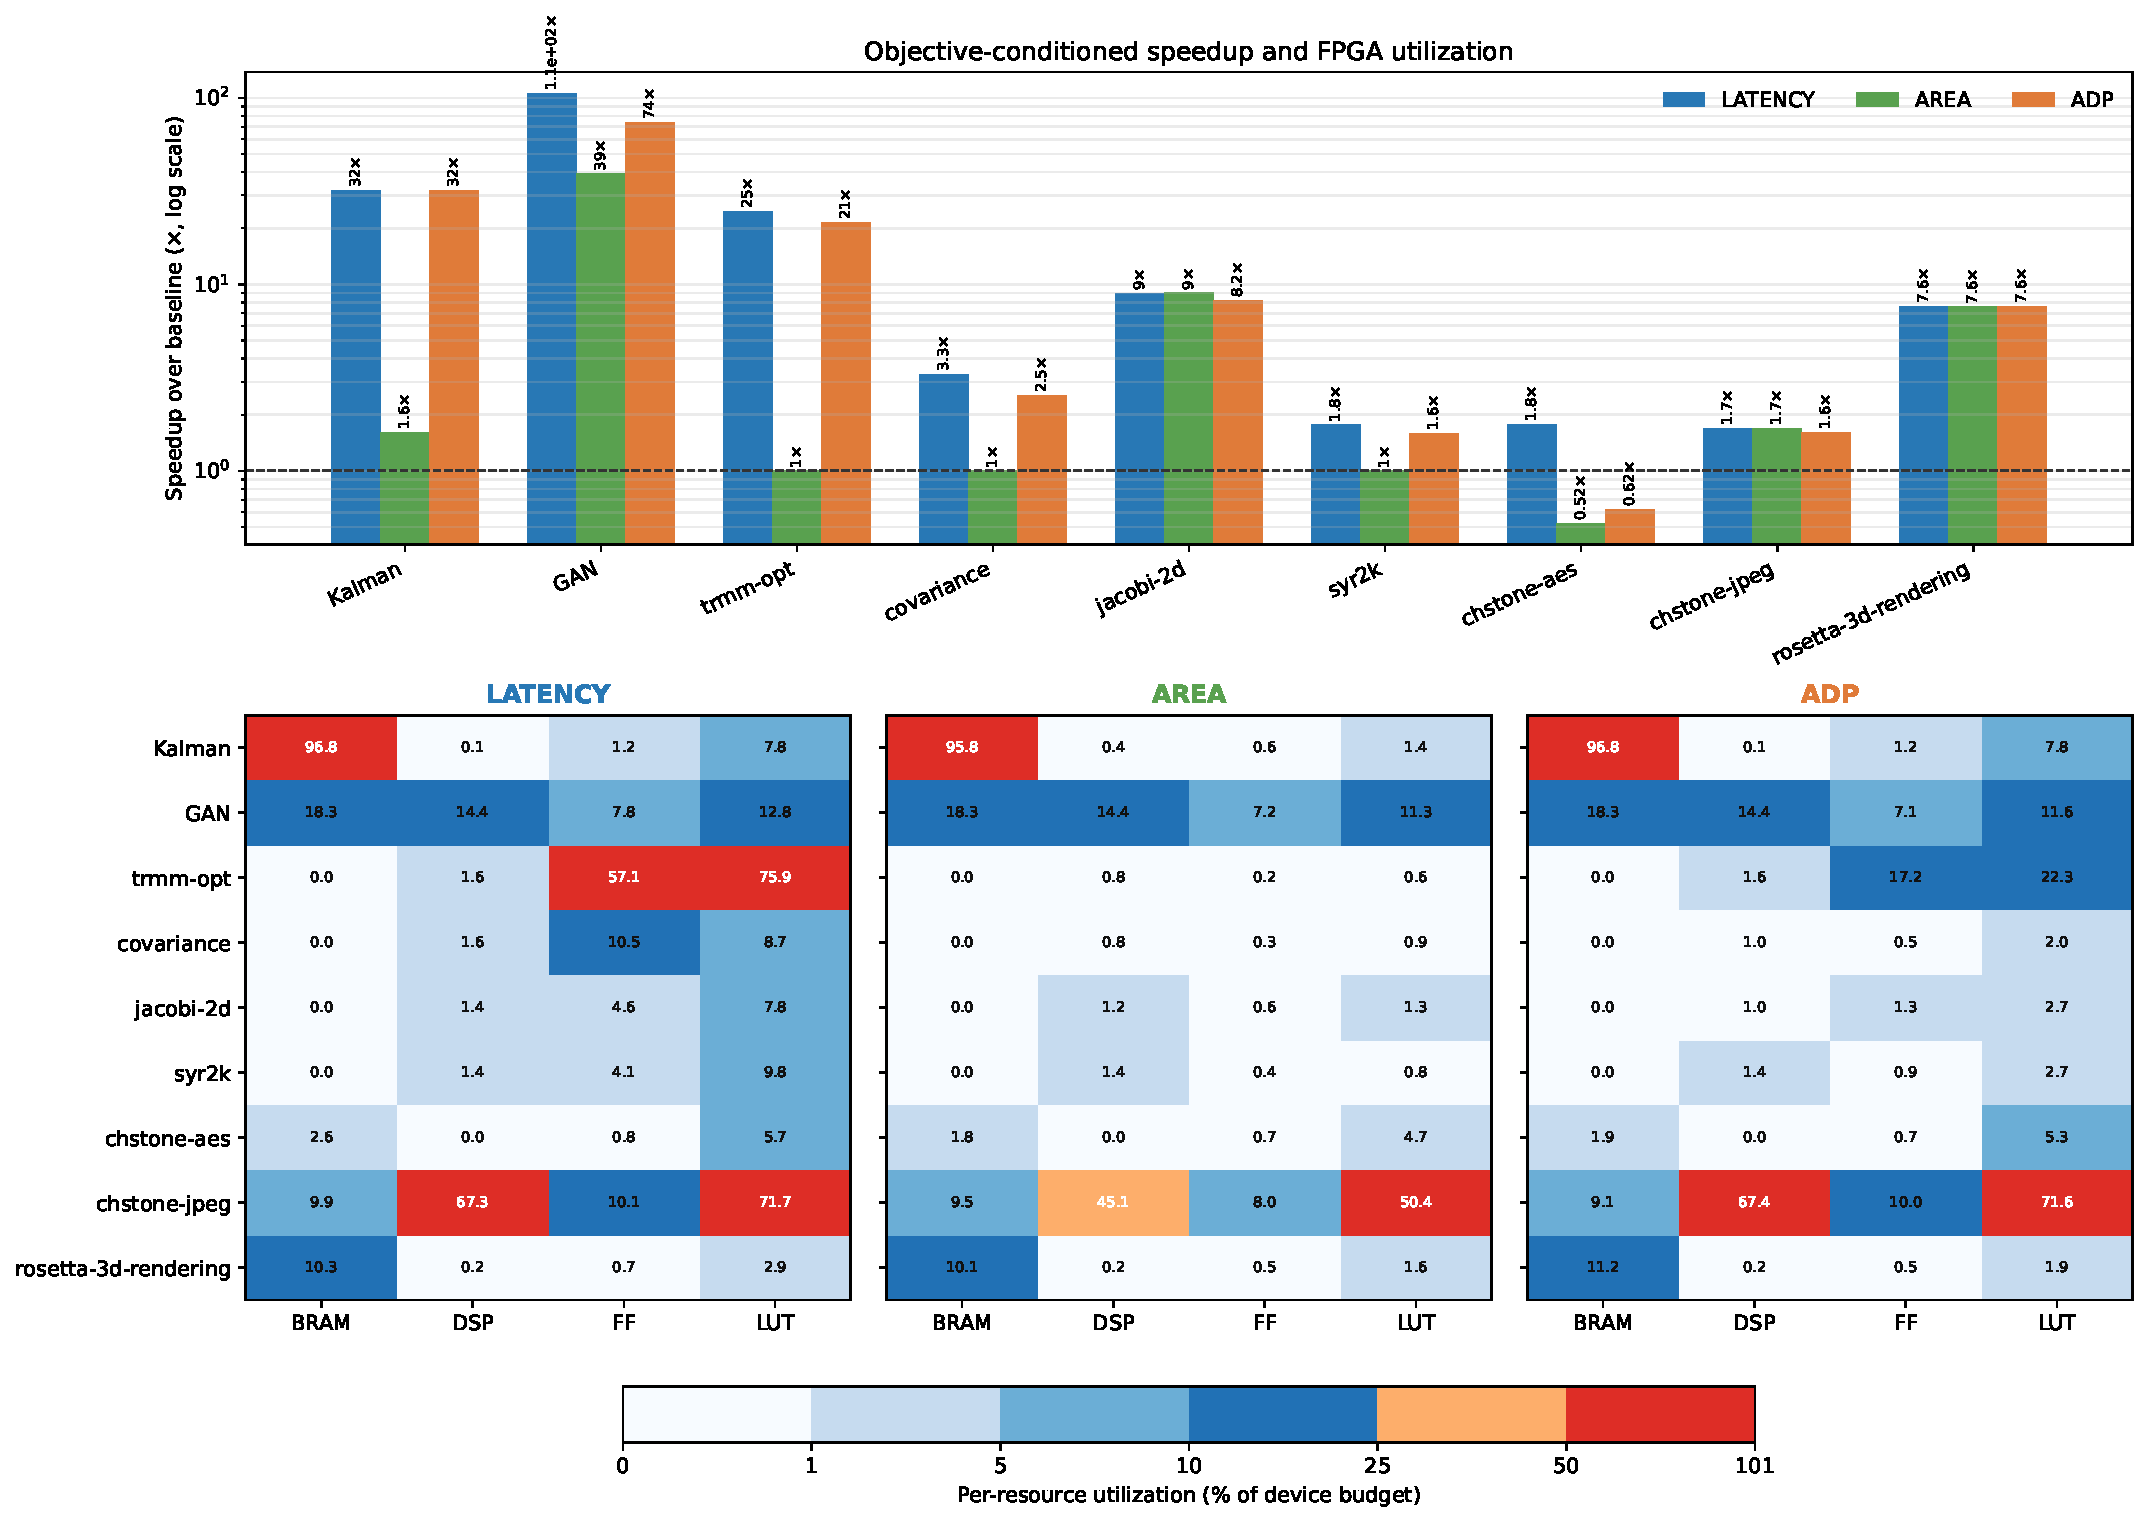
\includegraphics[
        width=0.96\textwidth
    ]{figures/04_Experimental/objective_speedup_resource_overview.pdf}
    \caption{
        \textbf{Objective-conditioned synthesized QoR across the evaluation suite.}
        Top: speedup over the corresponding pragma-free Vitis baseline for the
        latency-, area-, and ADP-oriented SALT-HLS policies.
        Bottom: per-resource BRAM, DSP, FF, and LUT utilization as a percentage
        of the target-device capacity for each objective.
        The results show that objective conditioning produces distinct
        performance--resource operating points rather than a single
        target-invariant directive policy.
    }
    \Description{
        Objective-conditioned SALT-HLS results across nine kernels.
        The upper panel compares latency, area, and ADP speedups over
        pragma-free Vitis on a logarithmic scale. Three lower heatmaps
        report BRAM, DSP, FF, and LUT utilization for the corresponding
        objective-specific designs.
    }
    \label{fig:objective-qor-overview}
\end{figure*}


\paragraph{End-to-end objective-conditioned QoR.}
Figure~\ref{fig:objective-qor-overview} evaluates the complete
SALT-HLS deployment path rather than prediction accuracy in
isolation. For every kernel, we fix the target (ZCU104/10\,ns),
resource capacity, source code, and legal directive action space,
and vary only the requested optimization policy. The latency, area,
and ADP models each emit one complete directive configuration
without online HLS feedback; the resulting design is synthesized
once to obtain the reported QoR. This setup therefore isolates two
questions central to SALT-HLS: whether a learned policy transfers
across heterogeneous workloads, and whether changing the objective
actually produces a different hardware optimization strategy rather
than a common directive template. All 27 objective-conditioned
designs reported in the figure satisfy the device resource limits.

Across the nine kernels, the latency policy achieves a
7.73$\times$ geometric-mean speedup over pragma-free Vitis.
The area policy reduces the suite-average area proxy $A$ from
14.61\% to 8.09\%---a 44.6\% reduction relative to the
latency policy---while retaining a 2.50$\times$ geometric-mean
speedup. ADP occupies the intended intermediate regime, reaching
6.16$\times$ at 10.88\% average $A$. The separation is expressed
primarily through FF and LUT consumption: their average utilization
falls from 10.76\%/22.57\% under latency optimization to
2.06\%/8.12\% under area optimization, whereas average BRAM
changes little. This is consistent with several workloads having a
memory footprint that forms a largely objective-independent floor,
while replication, scheduling, and control logic provide more freedom
for trading throughput against area.

The per-kernel spread also shows why optimization headroom cannot be
inferred from program size alone. GAN starts from a resource-light
baseline and exposes abundant regular compute parallelism, allowing
the latency policy to reach 105.39$\times$. Kalman represents the
opposite regime: its pragma-free implementation already consumes
97.1\% of ZCU104 BRAM, yet SALT-HLS reaches 31.81$\times$ while
using 96.8\% BRAM, i.e., the gain cannot be explained by simply
allocating more memory. Conversely, TRMM exposes only three directive
sites but reaches 24.62$\times$, whereas the structurally larger JPEG
kernel exposes 21 sites yet reaches only 1.70$\times$. Thus, the
number of available decisions is a poor proxy for achievable QoR:
the decisive factor is whether the program's dependence and memory
structure permits a few transformations to unlock useful parallelism.
The variation across Covariance (3.29$\times$), Jacobi-2D
(8.97$\times$), SYR2K (1.77$\times$), and TRMM
(24.62$\times$) makes the same point even within the regular
PolyBench class.

\paragraph{Directive-level policy specialization.}
The synthesized QoR differences correspond to substantial changes in
the directives themselves. Across the fixed 65 loop and 20 array
action sites, the latency policy enables pipelining at 50.8\% of loop
sites, non-trivial unrolling at 44.6\%, and array partitioning at
80.0\% of array sites. The area policy reduces these rates to
30.8\%, 12.3\%, and 40.0\%, respectively, and leaves both
pipeline and unroll disabled at 56.9\% of loop sites. ADP again lies
between the two, with 43.1\% pipelined loops, 32.3\% unrolled loops,
and 75.0\% partitioned arrays. Overall, the latency and area policies
select different complete directive assignments at 44 of the 85
action sites (51.8\%). Because the action locations and legal domains
are identical across objectives, this difference reflects learned
policy specialization rather than a change in the available search
space.

The specialization is microarchitecturally coherent rather than merely
statistical. On GAN, for example, the latency policy couples cyclic
partition factors of 15 and 25 on the hidden-layer buffers with
unroll factors of 30, 30, 15, and 25, reaching 105.39$\times$.
ADP narrows the corresponding banking to 5 and 5 and the unrolling
to 10, 10, 5, and 5, reaching 74.06$\times$; the area policy
reduces banking to factor 2 and removes explicit unrolling, reaching
39.10$\times$ with lower hardware cost. TRMM exhibits the same
ordering more sharply: the latency policy combines $20\times$
unrolling with two pipelined loops (24.62$\times$, $A=33.66\%$),
ADP uses $5\times$ unrolling and one pipeline
(21.48$\times$, $A=10.28\%$), while the area policy suppresses
these transformations and returns to the baseline-performance,
low-area regime ($1.00\times$, $A=0.42\%$). Importantly, more
aggressive directives are not always beneficial: on Jacobi-2D,
removing two $16\times$ unrolls preserves approximately
9$\times$ speedup while reducing $A$ from 3.47\% to 0.78\%.
Together, these cases indicate that SALT-HLS learns to coordinate
compute replication and memory bandwidth according to both the kernel structure and the requested objective, rather than applying a globally aggressive or conservative pragma recipe.





\subsection{Target generalization}
\label{subsec:target-generalization}

\subsubsection{Zero-shot Cross-Device and Cross-Frequency Transfer}
\label{subsubsec:zero-shot-target-transfer}

\begin{figure}[t]
    \centering
    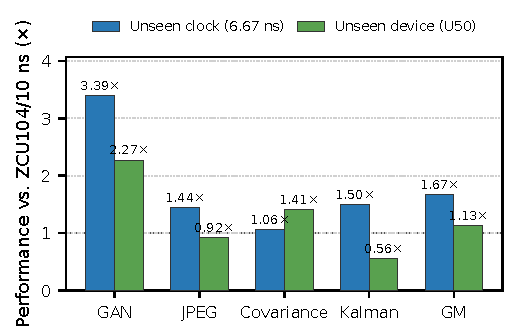
\includegraphics[
        width=0.98\columnwidth
    ]{figures/04_Experimental/target_generalization_zero_shot_qor-1.pdf}
\caption{
    \textbf{Zero-shot generalization to unseen deployment targets.}
    Starting from ZCU104/10\,ns, the frozen SALT-HLS latency policy is
    evaluated at an unseen 6.67\,ns clock and on an unseen U50 FPGA
    without retraining. Performance is normalized to the synthesized
    ZCU104/10\,ns SALT-HLS design using nominal execution time
    (cycles $\times$ requested period); values above $1\times$ indicate
    improvement over the source-target design. GM denotes the geometric
    mean across all four kernels.
}
\Description{
    Grouped bar chart reporting zero-shot performance relative to the
    ZCU104 10-nanosecond source-target SALT-HLS design for GAN, JPEG,
    Covariance, and Kalman. The two series correspond to an unseen
    6.67-nanosecond clock and an unseen U50 FPGA.
    }
    \label{fig:target-generalization}
\end{figure}

Figure~\ref{fig:target-generalization} asks a stricter question than
workload generalization: can the frozen policy respond to a deployment
target that was never observed during training? Starting from
ZCU104/10\,ns, we perturb one target dimension at a time. ZCU104/6.67\,ns
tests interpolation to an unseen clock between the trained 10 and 5\,ns
points, whereas U50/10\,ns changes the FPGA while holding the clock fixed.
The four kernels intentionally expose different target sensitivities.
GAN provides abundant coupled compute/memory parallelism (11 actions);
JPEG is the largest and most control/buffer-rich case (21 actions);
Covariance is a regular static-control kernel with only seven loop
actions; and Kalman has 13 actions, including six array decisions, while
its source-target design already occupies 96.8\% of ZCU104 BRAM. We retain
Kalman despite its negative U50 result precisely to expose the difficult
memory-constrained regime rather than selecting only favorable transfers.

The metric is execution-time improvement relative to the synthesized
ZCU104/10\,ns SALT-HLS design, not speedup over a pragma-free target
baseline. All four kernels benefit at the unseen clock, giving a
$1.67\times$ geometric mean. The mechanisms nevertheless differ:
GAN improves by $3.39\times$, as latency falls from 2,839 to 1,255 cycles
in addition to the shorter period; Kalman retains essentially the same
cycle count and therefore obtains the expected $1.50\times$ frequency
gain; JPEG tolerates a small cycle increase and still reaches
$1.44\times$; while Covariance grows from 59,643 to 84,671 cycles, nearly
cancelling the faster clock and yielding only $1.06\times$. Thus clock
transfer is useful but not equivalent to simply multiplying performance
by frequency: the HLS schedule and operator implementation may themselves
change under a different timing constraint.

Cross-device transfer is harder. U50 improves GAN and Covariance by
$2.27\times$ and $1.41\times$, respectively, but JPEG reaches
$0.92\times$ and Kalman $0.56\times$, giving a $1.13\times$ geometric
mean. The failures are informative rather than synthesis anomalies.
JPEG uses more aggressive parallelism on U50 yet increases DSP/FF/LUT
from 779/36.8K/116.1K to 1,159/60.2K/155.5K without reducing cycle
latency. Kalman similarly reorganizes its memory hierarchy but increases
latency from 327,772 to 589,818 cycles. Zero-shot device transfer
therefore does not guarantee that additional hardware parallelism matches
the kernel's actual bottleneck.


\paragraph{Directive response.}
The directives explain the asymmetric transfer behavior. At 6.67\,ns,
51 of the 52 action decisions remain unchanged; only one JPEG pipeline
decision changes. The intermediate timing target is therefore handled
largely by a portable source-target policy and by target-aware HLS
scheduling. U50 instead changes 17/52 actions (32.7\%). On GAN, SALT-HLS
doubles the cyclic banking of the two hidden-layer buffers
($15/25\!\rightarrow\!30/50$) together with the corresponding unroll
factors, a coherent memory/compute scaling that accompanies the
$2.27\times$ gain. JPEG raises two unroll factors from $2$ to $8$,
increases \texttt{QuantBuff} banking from $2$ to $8$, and completely
partitions two additional buffers, but this extra parallelism does not
translate to lower latency. Covariance requires no directive change and
still gains $1.41\times$, showing that its regular policy transfers
directly. Kalman changes 8/13 actions, doubling several partition and
unroll factors, yet performance regresses; its high source-target memory
pressure makes the useful hardware organization strongly device
dependent.

Overall, the experiment shows that target conditioning provides useful
zero-shot portability, but not universal target optimality. Frequency
interpolation is robust across all four workloads, whereas device transfer
depends more strongly on whether the source-level parallelization strategy
remains appropriate for the new hardware. The negative JPEG and Kalman
cases therefore delimit the zero-shot capability and motivate the
target-specific adaptation evaluated next.



\subsubsection{Post-Route Validation}
\label{subsubsec:postroute-validation}

Finally, we place and route all 12 designs underlying
Fig.~\ref{fig:target-generalization} with Vitis/Vivado 2021.1.
Table~\ref{tab:postroute-targets} reports the post-route critical-path
period. All designs fit the target FPGA and meet their requested clock,
including the unseen-target configurations.

\begin{table}[t]
    \centering
    \caption{\textbf{Post-route timing of the zero-shot designs (ns).}
    Column headers give the requested period; every reported period is
    below its corresponding target.}
    \label{tab:postroute-targets}
    \scriptsize
    \setlength{\tabcolsep}{3.2pt}
    \renewcommand{\arraystretch}{1.03}

    \begin{tabular}{lccc}
        \toprule
        & \textbf{ZCU104} & \textbf{ZCU104} & \textbf{U50} \\
        \textbf{Kernel}
        & \textbf{10 ns}
        & \textbf{6.67 ns}
        & \textbf{10 ns} \\
        \midrule
        GAN        & 6.289 & 4.830 & 6.908 \\
        JPEG       & 9.418 & 6.570 & 9.211 \\
        Covariance & 7.989 & 5.600 & 9.012 \\
        Kalman     & 8.381 & 6.238 & 9.097 \\
        \bottomrule
    \end{tabular}
\end{table}

This physical validation sharpens the interpretation of
Fig.~\ref{fig:target-generalization}. In particular, the negative U50
transfers for JPEG (0.92$\times$) and Kalman (0.56$\times$) still close
timing at 9.211 and 9.097\,ns, respectively. Their regressions therefore
come from increased cycle latency rather than failure to meet the target
clock. Conversely, all four unseen 6.67\,ns designs close timing---the
tightest is JPEG at 6.570\,ns---confirming that the observed
cross-frequency gains correspond to physically realizable implementations.
Post-route timing is used here as a feasibility check; performance remains
normalized using cycles times the requested period, as in
Fig.~\ref{fig:target-generalization}.



\subsubsection{Few-shot Adaptation to Uknown Device}

\EV{Include if good results sep 9 morning}


\subsection{Comparison with State-of-the-Art}
\label{subsec:sota-comparison}


\begin{figure*}[t]
    \centering
    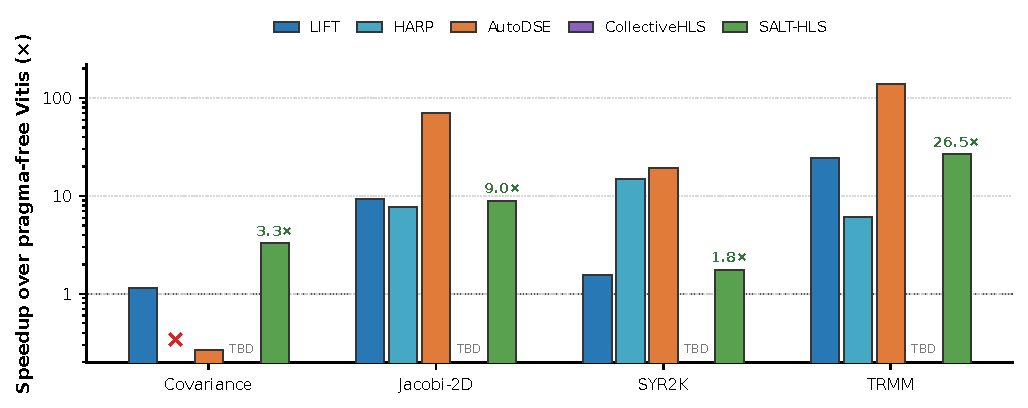
\includegraphics[
        width=0.82\textwidth
    ]{figures/04_Experimental/sota_common_kernels-2.pdf}
    \caption{
        \textbf{Comparison with state-of-the-art HLS optimization
        approaches on the common PolyBench kernels.}
        Speedup is measured over the same pragma-free Vitis baseline.
        A red $\times$ denotes a method for which no feasible synthesized
        design is available; ``n/e'' denotes a method--kernel pair not
        evaluated in the corresponding experiment, while ``TBD'' reserves
        the CollectiveHLS result currently being evaluated.
    }
    \Description{
        Grouped logarithmic bar chart comparing LIFT, HARP-DSE, AutoDSE,
        CollectiveHLS, and SALT-HLS on Covariance, Jacobi-2D, SYR2K,
        and TRMM.
    }
    \label{fig:sota-common}
\end{figure*}


\begin{figure}[t]
    \centering
    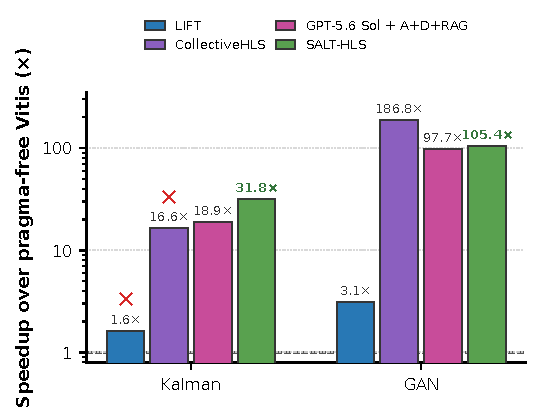
\includegraphics[
        width=0.98\columnwidth
    ]{figures/04_Experimental/sota_gan_kalman-3.pdf}
    \caption{
        \textbf{Comparison on fully unseen applications.}
        We compare SALT-HLS with LIFT, CollectiveHLS, and the strongest
        general-purpose LLM baseline, GPT-5.6 Sol under
        action-, domain-, and retrieval-augmented prompting.
        Speedup is measured over the pragma-free Vitis baseline.
        Red $\times$ markers denote synthesized configurations that violate
        FPGA resource constraints.
    }
    \Description{
        Logarithmic grouped bar chart comparing LIFT, CollectiveHLS,
        GPT-5.6 Sol with action-domain-RAG prompting, and SALT-HLS on
        the Serrano Kalman filter and GAN.
    }
    \label{fig:sota-external}
\end{figure}

\paragraph{Optimization Cost}


\begin{table}[t]
    \centering
    \caption{\textbf{Online optimization cost.}
    HLS calls used to guide optimization are separated from
    synthesis used only to validate the final selected design.
    Offline dataset construction and model training are excluded.}
    \label{tab:optimization-cost}

    \scriptsize
    \setlength{\tabcolsep}{2.5pt}
    \renewcommand{\arraystretch}{1.08}

    \begin{tabular}{lcccc}
        \toprule
        \textbf{Method} &
        \textbf{Search} &
        \textbf{HLS$_{\mathrm{fb}}$} &
        \textbf{HLS$_{\mathrm{val}}$} &
        \textbf{Online cost} \\
        \midrule

        AutoDSE~\cite{sohrabizadeh2020autodse}
        & $\sim$200
        & $\sim$200
        & incl.
        & 25\,h/kern. \\

        HARP-DSE~\cite{sohrabizadeh2023harp}
        & $\sim$100k
        & 0
        & 10
        & 1\,h + val. \\

        CollectiveHLS~\cite{ferikoglou2024collectivehls}
        & 1 prop.
        & 0$^\dagger$
        & 1$^\dagger$
        & 3.2\,s + HLS \\

        LIFT~\cite{prakriya2025lift}
        & 1 decode
        & 0
        & 1
        & N/R + HLS \\

        \textbf{SALT-HLS}
        & \textbf{1 decode}
        & \textbf{0}
        & \textbf{1}
        & \textbf{TBD + HLS} \\

        \bottomrule
    \end{tabular}

    \vspace{1pt}
    \parbox{0.98\columnwidth}{\scriptsize
    HLS$_{\mathrm{fb}}$: synthesis calls whose results guide
    configuration selection; HLS$_{\mathrm{val}}$: final
    measurement/validation synthesis.
    ``N/R'' denotes not reported.
    $^\dagger$CollectiveHLS can perform additional HLS calls when
    its directive re-proposal mechanism is activated.}
\end{table}


\subsection{Comparison with State of the Art}
\label{subsec:sota-comparison}

Figures~\ref{fig:sota-common} and~\ref{fig:sota-external} compare
SALT-HLS with complementary HLS optimization paradigms: synthesis-driven
DSE (AutoDSE), surrogate-guided DSE (HARP), direct LLM pragma generation
(LIFT), knowledge-driven transfer (CollectiveHLS), and a strong
general-purpose LLM. The comparison is intentionally split into two
sets because no baseline supports the same source/tool contract on all
applications. AutoDSE and HARP are released around Merlin-compatible
design spaces and databases~\cite{sohrabizadeh2020autodse,
sohrabizadeh2023harp}; we therefore evaluate them on the four common
PolyBench kernels. Their public flows require Merlin-compatible projects,
whereas GAN and Serrano-Kalman are external direct-Vitis applications,
so the latter panel uses baselines that can be applied to these sources.
These are consequently \emph{end-to-end framework comparisons under
each method's native directive space}, rather than a matched-action-space
ablation. AutoDSE's released implementation explicitly requires the
source project to run through Merlin, while HARP builds its DSE database
from AutoDSE/Merlin projects. \cite{sohrabizadeh2020autodse,
sohrabizadeh2023harp}

\paragraph{Common PolyBench kernels.}
Figure~\ref{fig:sota-common} exposes a clear quality--search-cost
trade-off. SALT-HLS reaches $3.29\times$, $8.97\times$,
$1.77\times$, and $24.62\times$ on Covariance, Jacobi-2D,
SYR2K, and TRMM, respectively, from a single generated configuration.
Its strongest relative result is Covariance: LIFT reaches
$1.14\times$, AutoDSE returns a $0.27\times$ configuration, and
HARP produces no feasible design among its physically validated
top-10 surrogate candidates. This case illustrates an advantage of
learning the configuration-selection policy directly: a surrogate
ranking can still concentrate its highest-ranked candidates in an
infeasible region, whereas SALT-HLS is trained from synthesized
target-feasible configurations and conditions the prediction explicitly
on the target resource limits.

The ranking reverses on Jacobi-2D and SYR2K. AutoDSE reaches
$70.32\times$ and $19.13\times$, while HARP reaches $7.64\times$
and $14.76\times$; on TRMM, AutoDSE reaches $139.19\times$,
substantially above both LIFT ($26.54\times$) and SALT-HLS
($24.62\times$). These gaps should not be interpreted as a failure of
structural grounding alone: the methods expose different optimization
spaces. Merlin combines \texttt{PIPELINE}, \texttt{PARALLEL}, and
\texttt{TILE} transformations and can derive lower-level memory
organization from these high-level choices, while SALT-HLS predicts
pipeline, unroll, and explicit array-partition actions learned from
GN$\Omega$SIS. AutoDSE can therefore exploit transformation
combinations that are absent or sparsely represented in SALT-HLS's
training support. This is particularly visible on SYR2K and TRMM,
where the best Merlin configurations use aggressive parallelization,
pipeline flattening, or tiling.

There is a concrete data limitation behind this distinction.
GN$\Omega$SIS represents each loop action by one categorical loop
directive, e.g., \texttt{pipeline\_1} or \texttt{unroll\_$k$}.
An exhaustive audit of our supplied multi-target training export
(1.11M loop-action instances) finds no example in which pipeline and
unroll are simultaneously active at the same action. Thus, although
the SALT-HLS output schema does not forbid such a combination, its
supervision provides no positive example from which to learn it. This
inherited support bias helps explain why search-based Merlin methods can
occasionally discover more aggressive configurations on regular
PolyBench nests. The public GN$\Omega$SIS schema likewise exposes one
loop-specific directive value per loop action. \cite{ferikoglou2026gnomegasis}

\paragraph{External GAN and Kalman applications.}
Figure~\ref{fig:sota-external} tests a different form of generalization:
the optimizers must operate on applications outside the common
PolyBench/Merlin comparison. On GAN, CollectiveHLS is strongest at
$186.8\times$, followed by SALT-HLS at $105.4\times$ and
GPT-5.6 Sol with action/domain/RAG prompting at $97.7\times$;
LIFT reaches $3.1\times$. GAN is a favorable case for transferring
aggressive parallelism: its regular dense computation exposes substantial
independent compute and memory-level parallelism. CollectiveHLS is
specifically designed to transfer directive distributions from
previously characterized applications with similar source-level
properties~\cite{ferikoglou2024collectivehls}, explaining why its
knowledge-based policy can be particularly effective on such a case.
The near-SALT performance of GPT-5.6 Sol is also informative: once
eligible actions, legal domains, and HLS guidance are supplied explicitly,
a strong general-purpose model can recover a competitive configuration
for a regular kernel.

Kalman separates the methods more sharply. SALT-HLS reaches
$31.81\times$ while remaining feasible at 96.8\% BRAM; GPT-5.6 Sol
reaches $18.9\times$, whereas CollectiveHLS ($16.6\times$) and
LIFT ($1.6\times$) exceed the resource limits. This is precisely the
regime in which target conditioning matters: the pragma-free Kalman
design already consumes 97.1\% of ZCU104 BRAM, leaving little tolerance
for an optimization policy that treats resource feasibility only
implicitly. LIFT is trained primarily for latency and explicitly does
not use resource utilization as an input supervision signal; invalid
designs are discouraged indirectly through their performance weight
~\cite{prakriya2025lift}. CollectiveHLS likewise optimizes latency from
transferred historical knowledge and its original evaluation already
identifies Kalman as an unseen-application feasibility failure
~\cite{ferikoglou2024collectivehls}. In contrast, SALT-HLS learns from
component-wise feasible targets and conditions every directive decision
on device, clock, BRAM/DSP/FF/LUT budgets, and objective. Its
action-aligned compiler memory further exposes the loop--memory relations
needed to coordinate unrolling with partitioning under the nearly
saturated BRAM constraint.

\paragraph{What does the comparison establish?}
No single optimizer dominates every kernel. Long-running DSE can exploit
a richer native transformation space and reaches the best latency on
several regular PolyBench kernels; knowledge transfer is exceptionally
strong on GAN. SALT-HLS instead provides a different operating point:
one objective- and target-conditioned directive configuration, no online
HLS feedback, and feasible synthesized outputs across the reported
comparisons. Its advantage is largest when optimization quality depends
on jointly reasoning about program structure and a binding hardware
constraint, as in Covariance and especially Kalman. Conversely, the
SYR2K/TRMM gaps expose an important limitation inherited from the
GN$\Omega$SIS supervision: direct prediction can only learn
transformation combinations adequately represented in its training
support. We therefore interpret SALT-HLS not as replacing exhaustive
search in every regime, but as substantially reducing online optimization
cost while retaining competitive QoR, explicit target awareness, and
robust feasibility across heterogeneous and external applications.





\section{Conclusion}

We presented \framework, a target-conditioned policy for HLS pragma optimization that combines source-derived directive domains with action-aligned compiler structure. The target-aware Stage~1 policy predicts directive values from source, objective, FPGA, component-wise resource budget, and clock; Stage~2 freezes that policy and injects QoR-supervised structured-MLIR embeddings only at directive decisions. This design makes task-specific fine-tuning and structural fusion independently measurable and avoids using GNN QoR predictions as an inference-time search oracle.

\resulttodo{Final 2--3 strongest quantitative conclusions from frozen ASPLOS checkpoints: main seen/unseen objective quality; validity/synthesis/resource-feasibility; cross-target evidence; and optimization/HLS-call cost.}

\paragraph{Limitations and future extensions.}
\framework predicts within source-derived loop/array directive domains instead of arbitrary source rewriting. Source-compatible predictions still require the HLS flow to verify timing, functionality, and resource feasibility. Generalization is also bounded by the devices, clocks, toolchain, and action-space sizes evaluated in this work. \asplostodo{State exactly which cross-device/frequency settings are zero-shot versus adapted and name untested toolchains explicitly. Mention broader directive space, additional FPGA families, and device-conditioned structural encoders only as future work.}


% ASPLOS'27/ACM requires full disclosure of generative-AI use. This section is excluded from the 11-page limit when used for this purpose.
\section*{Acknowledgments}
OpenAI ChatGPT was used to assist with editing author-provided prose and checking the manuscript against the authors' stated revision plan. The authors determined the research questions and methodology, performed the implementation and experiments, selected the reported evidence, and are responsible for verifying all technical claims, citations, and final text.

\bibliographystyle{ACM-Reference-Format}
\bibliography{refs-base,refs-gnn-papers,refs-llm-papers,refs-synthesis-based-papers,refs-asplos-update}

\end{document}
